\documentclass[english, msc, oneside]{layout/observatory-thesis}
\usepackage[utf8]{inputenx}

\usepackage{algorithm}
\usepackage{algpseudocode}
\usepackage{mathtools}
\usepackage{MnSymbol}


\usepackage{graphicx} 
\usepackage{amsmath,amssymb,amsthm}

\usepackage{mdframed}
\usepackage{lipsum}

\theoremstyle{definition}
\newtheorem{exmp}{Example}[section]
\newtheorem{theorem}{Theorem}[section]
\newtheorem{corollary}{Corollary}[theorem]
\newtheorem{lemma}[theorem]{Lemma}

\newmdtheoremenv{theo}{\textbf{Results}}


\begin{document}


\title{\textbf{On the Stable Matching \\Lattices}}
\subtitle{Structure and Representation of all Stable Matchings} 
\subject{\thesistypeshort thesis}
\author{Argha Sardar}
\studentid{21510035}
\supervisor{Dr. Neeldhara Misra}
\projectstart{August 2022}
\projectend{April 2023}
\affiliation{Discipline of Mathematics, IIT Gandhinagar}
\address{Indian Institute of Technology, Gandhinagar, Gujarat 382355, India}
\coverimage{layout/figures/free_frontpage/1.jpg}
\covercredit{Night sky by John Fowler} 

\frontmatter 

\makecover 
\maketitle 

\dedication{Dedicated to my Maa and Baba who believed in me.}

\disclaimer

\chapter{Abstract}

The focal point of this thesis is the lattices of stable matching, in conjunction with their structures and representations. The introduction of foundational concepts such as matchings, poset, and lattices marks the beginning of the thesis, culminating in the presentation of the stable marriage problem. The enduring fascination with stable matching problems has garnered interest among numerous professionals, including computer scientists, mathematicians, and economists, ever since their inception by \textit{Gale} and \textit{Shapley} in 1962. In spite of the passage of time, the allure of stable matching problems continues to mount. Recent years have seen a dramatic upswing in our understanding of these problems, our proficiency in resolving them, and our appreciation of their structural interplay with other combinatorial problems.

The next two chapters focuses on the stable marriage problem with monogamous matchings of equal numbers of men and women, where each person's list contains all individuals of the opposite sex and all preferences are strict. The chapter presents a powerful and algorithmically revealing representation of the set of all stable matchings and the marriage lattice $\mathcal{M}$ for any problem instance. Despite the possibility of an exponential growth in the number of stable matchings, for any instance of size $n$, there exists a partial order $\Pi(\mathcal{M})$ with $O(n^2)$ elements that represents all stable matchings. The set of closed subsets of $\Pi(\mathcal{M})$, defined later, corresponds to the set of stable matchings in $\mathcal{M}$ in a one-to-one manner. Furthermore, the relationship of set containment on the closed subsets of $\Pi(\mathcal{M})$ is the dominance relation on the corresponding stable matchings. The chapter demonstrates how $\Pi(\mathcal{M})$ can be constructed efficiently from preference lists without knowing $\mathcal{M}$.

The compact representation of the set of all stable matchings, as well as the partial order $\Pi(\mathcal{M})$, will be essential to efficient algorithms for a range of stable marriage problems. The partial order $\Pi(\mathcal{M})$ can be used to establish complexity results through problem reductions and to demonstrate the stable marriage problem's relationship to various other well-known problems in combinatorial optimization.

\chapter{Acknowledgements}

I would like to express my deepest gratitude to my supervisor, \textbf{Prof. Neeldhara Misra}, for her guidance, encouragement, and invaluable feedback throughout the writing process of this thesis. I am also grateful to the members of my thesis committee, \textit{Prof. Indranath Sengupta}, \textit{Prof. Sanjay Amrutiya}, and \textit{Prof. Projesh Nath Choudhury}, for their insightful comments and suggestions.

I want to thank \textbf{Prof. Ashutosh Rai} from \textit{IIT Delhi} for his weekly lecture series on Stable Matching, which helped me tremendously in completing my thesis. His expertise and dedication were invaluable, and I am grateful for his support.
I would like to thank my colleagues at \textit{IIT Gandhinagar} for their support, especially \textit{Ms. Saraswati Nanoti}, \textit{Mr. Harshil Mittal}, and \textit{Mr. Anant Kumar}, who have helped me with understanding proofs wherever I stumbled upon and provided valuable insights into my research.

I am grateful to my family for their unwavering love and support, especially my parents, who have encouraged me to pursue my academic dreams and believed in me even when I doubted myself.

They say that behind every successful student is a group of friends who kept them sane, and I can't thank my squad enough for doing just that. They listened to me complain about endless readings and deadlines, celebrated my small victories, and always had a joke or two to lift my spirits. I don't know how I would have survived this journey without their friendship, and I feel lucky to have them in my life. Here's to more laughs, adventures, and academic triumphs together! And specially thanks to \textit{Rik Da} and \textit{Sohini Di}, who were there for me when nobody else was. Their unwavering support and presence lifted me up in moments of solitude and uncertainty. I am forever grateful for the memories we created together.
\newline

Thank you all for your contributions to my success.
\bigskip

\begin{flushright}   \textbf{ARGHA SARDAR}, 21510035 \\ \textit{IIT Gandhinagar} \\ April, 2023 \end{flushright}

\tableofcontents


\mainmatter 

\chapter{Stable Matching}

\section{Introduction}

\subsection{Matching}

    A \textbf{Matching} of \textit{graph}, $G$ is a \textit{subgraph} $M \subseteq G$ such that every edge shares no vertex with any other edge. That is, each vertex in matching $M$ has  degree \textbf{one}.
     
    The \textbf{size} of a matching is the number of edges in that matching.

\begin{figure}[ht]
    \begin{center}
  \includegraphics[width=0.4\textwidth]{IMAGES_FIGS/FIG_1_1.png}
  \caption{A Graph $G$ with $8$ vertices and $9$ edges.}
  \label{FIG_1_1}
  \end{center}
  
\end{figure}

In Figure \ref{FIG_1_1}, let's denote the edge that connects vertices $i$ and $j$ as $(i, j)$. Note that $\{(3, 8)\}$ is a \textit{matching}. The pairs $\{(3, 8),(4, 7)\}$ also make a \textit{matching} which is of size \textit{two}. Can we get a matching of size three? \textbf{Yes} !!!, it is $\{(2, 3),(4, 8),(5, 7)\}$. 


\subsection{Maximal matching}
    \begin{figure}[ht]
    \begin{center}
  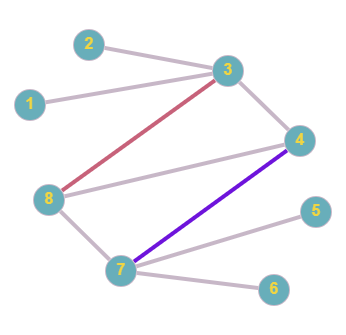
\includegraphics[width=0.4\textwidth]{IMAGES_FIGS/FIG_1_2.png}
  \caption{Coloured edges denoting the \textit{Maximal matching}}
  \label{FIG_1_2}
  \end{center}
  
\end{figure}

A \textbf{maximal matching} is a matching $M$ of the graph $G$, that is not a \textit{subset} of any other $matching$.
       
\textit{Example:} $\{(3, 8),(4, 7)\}$, It can't be a subset of any other Matching.
 

\subsection{Maximum matching}

A matching is \textbf{maximum} when it has the largest possible size. The \textbf{matching number} of a graph $G$ is the size of a \textit{maximum matching} of that graph.

    \begin{figure}[ht]
    \begin{center}
  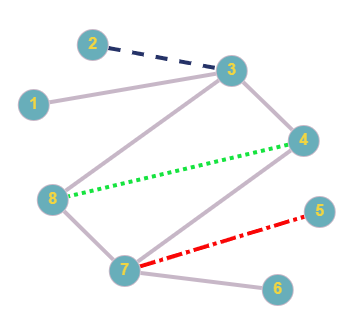
\includegraphics[width=0.4\textwidth]{IMAGES_FIGS/FIG_1_3.png}
  \caption{Coloured edges denoting the \textit{Maximum matching}}
  \label{FIG_1_3}
  \end{center}
  
\end{figure}


\textit{Note}: The \textbf{matching number} of the graph in Figure \ref{FIG_1_3} is $three$.
\newline
For a given graph $G$, there might be several \textit{maximum matchings}.
 

\subsection{Perfect Matching}

A matching $M$ of a graph $G$ is \textbf{perfect} if it contains all of the graph $G^\prime s$ vertices. 
That is, a matching is perfect if every vertex of the graph is incident to an edge of the matching. Every perfect matching is maximum and hence maximal.
\newline
\textit{Note} : \textbf{No perfect} matching exists for Figure \ref{FIG_1_4}.
\begin{figure}[ht]
\begin{center}
  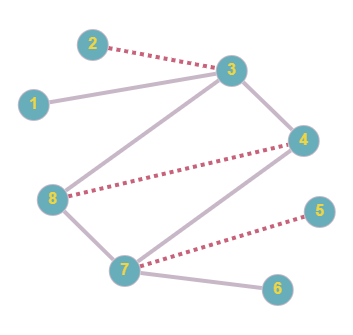
\includegraphics[width=0.4\textwidth]{IMAGES_FIGS/FIG_1_4.png}
  \caption{Dotted edges denoting the \textit{Perfect matching}}
  \label{FIG_1_4}
  \end{center}
  
\end{figure}

Well, a matching of size four means that every vertex is paired, but vertices $1$ and $2$ must both be paired with vertex $3$. So no, three is the best we can do. We call it a maximum matching.
 

\section{The Stable Marriage problem}
The \textbf{stable marriage problem} \textit{(SM)} describes the problem of finding a stable matching between two distinct, equally sized sets of players with complete preferences (namely \textbf{instances})\cite{gusfield_irving_1989}.
 
\subsection{The Game}
Consider two distinct sets, $\mathbb{M}$ and $\mathbb{W}$, each of size $\mathbf{N}$, and let us refer to these sets as the set of men and women respectively. Each element of $\mathbb{M}$ and $\mathbb{W}$ has a ranking of all the other set`s element associated with it, and we call this ranking as their preference list.
 
 

\subsection{The Stable Marriage Problem }
We can consider the preference lists for the elements of each set as a function which produces tuples. We call these functions $f$ and $g$ respectively:
$$f:\mathbb{M} \longrightarrow \mathbb{W}^N$$
$$g:\mathbb{W} \longrightarrow \mathbb{M}^N$$
This construction of men, women and their preference lists is called a game of size $N$, and is denoted by $(\mathbb{M}$,$\mathbb{W})$. This game is used to model instances of \textit{stable marriage}.
 
\subsection{Preference list}
Each person's preference list is a \textbf{ranking} over all of the members of the opposite sex.
\begin{center}
\begin{tabular}{ cc }   % top level tables, with 2 columns
% leftmost table of the top level table
\begin{tabular}{ |c||c|c|c|c|c|c|c| } 
\hline
1 & 5 & 7 & 1 & 2 & 6 & 3 & 4 \\
\hline
2 & 1 & 5 & 7 & 4 & 6 & 3 & 2 \\
\hline
3 & 7 & 3 & 5 & 1 & 2 & 6 & 4 \\
\hline
4 & 3 & 4 & 6 & 2 & 1 & 7 & 5 \\
\hline
5 & 7 & 1 & 5 & 3 & 2 & 6 & 4 \\
\hline
6 & 4 & 6 & 2 & 1 & 3 & 5 & 7 \\
\hline
7 & 5 & 7 & 1 & 3 & 6 & 4 & 2 \\
\hline
\end{tabular} &  % starting rightmost sub table
% table 2
\begin{tabular}{ |c||c|c|c|c|c|c|c| } 
\hline
1 & 4 & 3 & 5 & 2 & 6 & 1 & 7 \\
\hline
2 & 3 & 2 & 6 & 7 & 1 & 5 & 4 \\
\hline
3 & 2 & 1 & 7 & 6 & 5 & 3 & 4 \\
\hline
4 & 1 & 7 & 3 & 6 & 2 & 5 & 4 \\
\hline
5 & 5 & 6 & 4 & 3 & 2 & 1 & 7 \\
\hline
6 & 6 & 4 & 1 & 3 & 7 & 5 & 2 \\
\hline
7 & 7 & 5 & 1 & 3 & 6 & 2 & 4 \\
\hline
\end{tabular} \\ \\
Men's Preferences & Women's Preferences \\ 
\end{tabular}
\begin{figure}[ht]
  \caption{A stable matching instance of size $7$}
  \label{FIG_1_5}
\end{figure}
\end{center}

\subsection{The Matching}
    A matching ${M}$ is any \textbf{bijection} between $\mathbb{M}$ and $\mathbb{W}$. If a pair $(m,w) \in \mathbb{M} \times \mathbb{W}$ are matched in $M$, then we say that $p_M(m) = w$ and, equivalently, $p_M(w) = m$.
 

\subsection{Preference}
    Let $\mathbb{(M}$,$\mathbb{W)}$ be an instance of SM. Consider $m\in \mathbb{M}$ and $w,w^\prime \in \mathbb{W}$. We say that the man  $m$ prefers $w$ to $w^\prime$ if $w$ appears before $w^\prime \in f(m)$. The definition is equivalent for Women's preference list too\cite{dickerson}.
 
\subsection{Stability}
\textbf{Blocking Pairs : } A pair $(m,w)$ is said to \textbf{block} a matching $M$ if all of the following hold:
    \begin{enumerate}
  \item $m$ and $w$ arent matched in $M$, i.e. $p_M(m) \neq w$.
  \item $m$ prefers $w$ to $p_M(m) = w^\prime$.
  \item $w$ prefers $m$ to  $p_M(w) = m^\prime$ 
\end{enumerate}


\begin{center}
\begin{tabular}{ cc }   % top level tables, with 2 columns
% leftmost table of the top level table
\begin{tabular}{ |c||c|c|c|c| } 
\hline
1 & 4 & 1 & 2 & 3\\
\hline
2 & 2 & 3 & 1 & 4\\
\hline
3 & 2 & 4 & 3 & 1\\
\hline
4 & 3 & 1 & 4 & 2\\
\hline
\end{tabular} &  % starting rightmost sub table
% table 2
\begin{tabular}{ |c||c|c|c|c| } 
\hline
1 & 4 & 1 & 3 & 2\\
\hline
2 & 1 & 3 & 2 & 4\\
\hline
3 & 1 & 2 & 3 & 4\\
\hline
4 & 4 & 1 & 3 & 2\\
\hline
\end{tabular} \\ \\
Men's Preferences & Women's Preferences
\end{tabular}
\begin{figure}[ht]
  \caption{A stable marriage instance of size $4$}
  \label{FIG_1_7}
\end{figure}
\end{center}
\textit{Note} : The matching $\{(1,3),(2,4),(3,2),(4,1)\}$ doesn't forms a stable matching, as because $(1,4)$ and $(2,3)$ forms a blocking pair.
 
But, $\{(1,4),(2,3),(3,2),(4,1)\}$ forms a stable matching.

 
\subsection{Stable Matching}
A matching $M$ is said to be \textbf{stable} if it contains \textbf{no blocking pairs}, and unstable otherwise.
 
A man $m$ and a woman $w$ constitute a \textbf{stable pair} if and only if $m$ and $w$ are partners in some stable matching $M$.
 
If some man $m$ and woman $w$ are partners in all stable matchings, then $(m, w)$ is called a \textbf{fixed pair}.
 
 

\subsection{Algorithm : Stability Check}
\begin{center}
\begin{minipage}{.7\linewidth}
\begin{algorithm}[H]
\caption{Stability checking algorithm}
\begin{algorithmic}[1]
\For {$m \coloneqq 1,2,\ldots n$}
	\For {each $w$ such that $m$ prefers $w$ to $p_M(m)$}
	    \If {$w$ prefers $m$ to $p_M(w)$ }
		    \State report matching unstable
		    \State halt
		\EndIf
	\EndFor
\EndFor
\State report matching stable
\end{algorithmic}
\end{algorithm}
\end{minipage}
\begin{figure}[ht]
  \caption{Stability checking algorithm}
  \label{FIG_1_6}
\end{figure}
\end{center}


\section{The Gale \& Shapley's Algorithm}

In 1962, \textbf{David Gale} and \textbf{Lloyd Shapley} proved that every instance of the \textbf{Stable marriage problem} admits at least one stable matching. Gale and Shapley proved this result by describing an algorithm that is guaranteed to find such a matching. Furthermore, Gale and Shapley showed that their algorithm  simultaneously gives all the men (or all the women, if the roles of the sexes are reversed) the best partner that they can have in any stable matching\cite{marden}. 

\subsection{The Algorithm}

\begin{center}
\begin{minipage}{.9\linewidth}
\begin{algorithm}[H]
\caption{The Gale-Shapley algorithm}
\begin{algorithmic}[1]

\State Assign each person to be free
\While{some man $m$ is free}
    \State $w$ $\coloneqq$ first woman on $m$'s list to whom $m$ has not yet proposed\;
    \If {$w$ is free}
        \State assign $m$ and $w$ to be engaged {to each other}
    \Else
        \If {$w$ prefers $m$ to her fiancé $m_0$}
            \State assign $m$ and $w$ to be engaged and $m_0$ to be free
        \Else
            \State $w$ rejects $m$ {and $m$ remains free}
        \EndIf
    \EndIf
\EndWhile
\State output the stable matching consisting of the $n$ engaged pairs
\end{algorithmic}
\end{algorithm}
\end{minipage}
\begin{figure}[ht]
  \caption{The Gale \& Shapley's Algorithm}
  \label{FIG_1_8}
\end{figure}

\end{center}

\subsection{Some questions}
\begin{itemize}
\item Does a stable solution to the marriage problem always exist?
\item Can we compute such a solution efficiently?
\item Can we compute the best stable solution efficiently?
\end{itemize}

\subsection{Some Questions : Algorithm Termination}

\begin{theorem}\label{thm_1_1}
Gale-Shapley's Algorithm terminates in polynomial time (at most $n^2$ iterations of the outer loop).
\end{theorem}

\begin{proof}
Consider the following \textit{observations}:
\begin{enumerate}
\item Once a woman has a proposal, she will always have a proposal
\item If at least one woman has no proposals, then there exists at least one woman that has
multiple proposals.
\item Suppose every woman has at least one proposal, then every woman has exactly one
proposal and the Gale-Shapley algorithm terminates.
\end{enumerate}
\end{proof}

\subsection{Some Questions : Algorithm's running time}\label{thm_1_2}

\begin{theorem}
    If there are $n$ men and women, the Gale-Shapley algorithm terminates in atmost $n^2 - n + 1$ rounds.
\end{theorem}

\begin{proof}
    Since the algorithm’s input is a pair of $n \times n$ matrices
    \begin{enumerate}
        \item \textbf{Observations}
        \begin{enumerate}
            \item A man can get rejected at most $n-1$ times
            \item Every non-terminal stage there is at least one rejection
            \item Every woman will receive a proposal before termination
        \end{enumerate}
           
        \item \textbf{Proof}
        \begin{enumerate}
            \item \textbf{Initial proposal} : 1 stage
            \item Suppose every man gets rejected exactly $n-1$ times: $n\cdot(n-1)$ stages
            \item \textbf{Final proposal} : 1 stage
            \item Total number of stages \textit{(worst-case)}: ${n\cdot(n-1)}+1 = n^2-n+1$
        \end{enumerate}
    \end{enumerate}
\end{proof}

\subsection{The worst case instance}
Consider an instance of $n$ men and women where their choices are positioned a following manner.
\begin{center}
\begin{tabular}{ cc }   % top level tables, with 2 columns
\begin{tabular}{ |c || c c c c c| } 
\hline
$1$ & $1$ & $2$ & \ldots & $n-1$ & $n$\\
\hline
$2$ & $2$ & $3$ & \ldots & $1$ & $n$\\
\hline
$3$ & $3$ & $4$ & \ldots & $2$ & $n$\\
\hline
\ldots & & & \ldots & & \\
\hline
$n-1$ & $n-1$ & $1$ & \ldots & $n-2$ & $n$\\
\hline
$n$ & $1$ & $2$ & \ldots & $n-1$ & $n$\\
\hline
\end{tabular} &  % starting rightmost sub table
% table 2
\begin{tabular}{ |c || c c c c c| } 
\hline
$1$ & $2$ & $3$ & \ldots & $n$ & $1$\\
\hline
$2$ & $3$ & $4$ & \ldots & $1$ & $2$\\
\hline
$3$ & $4$ & $5$ & \ldots & $2$ & $3$\\
\hline
\ldots & & & \ldots & & \\
\hline
$n-1$ & $n$ & $1$ & \ldots & $n-2$ & $n-1$\\
\hline
$n$ & $1$ & $2$ & \ldots & $n-1$ & $n$\\
\hline
\end{tabular}\\ \\
Men's Preferences & Women's Preferences \\
\end{tabular}

\begin{figure}[ht]
  \caption{Worst Case}
  \label{FIG_1_9}
\end{figure}

\end{center}

\textit{Note :} In the instance specified by the preference lists in the above table, if the men begin their proposal sequences in strict numerical order, and the implementation strategy described above, involving a stack, is followed, then it may be verified that the $i^{th}$ proposal is from man $((i-1) \mod\:n) + 1$ to woman $((i-1) \mod(n-1))+1$, for $i = 1, \ldots n^2-n$, and the last proposal is from man $1$ to woman $n$.

\subsection{Some Questions : Perfect matching}

\begin{theorem}\label{thm_1_3}
    Gale-Shapley's Algorithm results in a perfect matching
\end{theorem}

\begin{proof}
    Let's proof by the method of contradiction : 
\begin{enumerate}
    \item WLOG let $m$ is unmatched at termination.
    \item $\longrightarrow$ there exist another women $w$ who is still unmatched upon termination of the Gale Shapley's Algorithm.
    \item Once a woman is matched, she is never unmatched; she only swaps partners. Thus, nobody proposed to $w$.
    \item But, the man $m$ proposes to every woman, since $m$ ends up unmatched.
    \item Now, at any stage since $w$ was unmatched $m$ must have proposed to $w$ and, she should have accepted that proposal : By \textbf{GS algorithm}.
\end{enumerate}
So, a contradiction arises which results into a perfect matching.
\end{proof}

\subsection{Stability}

\begin{theorem}\label{thm_1_4}
    The Gale-Shapley's Algorithm results in a stable matching (i.e., there are no blocking pairs).
\end{theorem}

\begin{proof}
    Assume $m$ and $w$ form a blocking pair
\begin{enumerate}
    \item \textbf{CASE} : $m$ never proposed to $w$
    \begin{enumerate}
        \item $GS:$ men proposes in order of preferences
        \item $m$ prefers current partner $w^\prime > w$
        \item $\longrightarrow$ $m$ and $w$ are not blocking
    \end{enumerate}
       
    \item \textbf{CASE} : When $m$ proposed to $w$
    \begin{enumerate}
        \item $w$ rejected $m$ at some point
        \item $GS:$ women only reject for better partners
        \item $w$ prefers current partner $m^\prime > m$
        \item $\longrightarrow$ $m$ and $w$ are not blocking
    \end{enumerate}
\end{enumerate}
Case $\#1$ and $\#2$ exhaust space, hence contradiction so no blocking pair arises.
\end{proof}

\subsection{Man Optimal and Pessimal}
Let's ask some question regarding man optimality and pessimality
    \begin{enumerate}
        \item Let $\mathbb{S}$ be the set of stable matchings.
        \item $m$ is a \textbf{valid partner} of $w$ if there exists some stable matching $S$ in $\mathbb{S}$ where they are paired.
    \end{enumerate}
A matching is \textbf{Man-optimal} if each man receives his \textbf{best valid} partner.
    \begin{enumerate}
        \item Is this a perfect matching?
        \item Is this a stable matching?
    \end{enumerate}
A matching is \textbf{Man-pessimal} if each man receives his \textbf{worst valid} partner.
    \begin{enumerate}
        \item Is this a perfect matching?
        \item Is this a stable matching?
    \end{enumerate}

\subsection{Man Optimal}

\begin{theorem}\label{thm_1_5}
    \textit{Gale-Shapley} : with the man proposing results in a \textit{man optimal} matching
\end{theorem}

\begin{proof}
Let's proof using the method of contradiction.
    \begin{enumerate}
    \item Men proposes in order, let at least one man was rejected by a valid partner.
    \item Let $m$ and $w$ be the first such pair to get rejected in $S$, \\ ($m$ and $w$`s engagement gets jilted)
    \item Happens because $w$ is matched with some $m^\prime > m$
    \item Let $S^\prime$ be a stable matching with $m, w$ paired
    \item Let $w^\prime$ be partner of $m^\prime$ in $S^\prime$
    \item $m^\prime$ was not rejected by valid woman in S before $m$ was rejected by $w$ \\ (by assump.) $\longrightarrow$ $m^\prime$  prefers $w$ to  $w^\prime$ 
    \item But $w$ prefers $m^\prime$ over $m$, her partner in $S^\prime$ $\longrightarrow$ $m^\prime$ and $w$ forms a blocking pair in $S^\prime$
\end{enumerate}
Hence, a contradiction arises which affects the stability of matching, so our claim is verified.\cite{The_SMP}
\end{proof}

\subsection{Woman Pessimal}

\begin{theorem}
    \textit{Gale-Shapley} : with the man proposing results in a \textit{woman pessimal} matching
\end{theorem}

\begin{proof}\label{thm_1_6}
Let's proof using the method of contradiction.
    \begin{enumerate}
    \item Let us assume $m$ and $w$ matched in $S$, $m$ is not worst valid
    \item $\longrightarrow$ there exists a stable matching $S^\prime$ with $w$ paired to $m^\prime < m$
    \item Let us consider $w^\prime$ be a partner of $m$ in $S^\prime$
    \item $m$ prefers to $w$ to $w^\prime$ (by Man optimality)
    \item $\longrightarrow$ $m$ and $w$ forms blocking pair in $S^\prime$
\end{enumerate}

Hence, a contradiction arises which affects the stability of matching, so our claim is verified
\end{proof}


\section{Lattices of stable Matching}

\subsection{The Dominance}
For a general stable marriage instance, the man optimal and woman optimal solutions are extreme stable matchings in a very precise sense, and that, in general, other stable matchings may also exist.\cite{gusfield_irving_1989} 

A person $x$ is said to prefer a matching $M$ to a matching $M^\prime$, if $x$ prefers his/her partner in $M$ to his/her partner in $M^\prime$. Note that this is strict preference. Given two stable matchings $M$ and $M^\prime$, a person $x$ may prefer $M$ to $M^\prime$, or $M^\prime$ to $M$, or may, if $p_M(x) = p_{M^\prime}(x)$, be indifferent between them.

\subsection{Dominance Example}

\begin{itemize}
    \item  The Man number $1$ prefers the matching $M$ to $M^\prime$ when his partner in $M$ is ranked higher than his partner in $M^\prime$ (w.r.t. Man $1$'s preference list) i.e. Man $1$ prefers the Women $1$ more than Women $2$.
    \item Similarly the Man number $2$ prefers the matching $M^\prime$ to $M$ when his partner in $M$ is ranked lower than his partner in $M^\prime$ (w.r.t. Man $2$'s preference list) i.e. Man $2$ prefers the Women $4$ more than Women $2$.
    \item Man $3$ has indifferent choices between his partner in matching $M$ and $M^\prime$
\end{itemize}
\pagebreak

\begin{center}
\begin{tabular}{ cc }   % top level tables, with 2 columns
  
% leftmost table of the top level table
\begin{tabular}{ |c||c| } 
\hline
1 & 1 \\
\hline
2 & 2 \\
\hline
3 & 3\\
\hline
4 & 4\\
\hline
\end{tabular} &  % starting rightmost sub table
% table 2
\begin{tabular}{ |c||c| } 
\hline
1 & 2 \\
\hline
2 & 4 \\
\hline
3 & 3\\
\hline
4 & 1\\
\hline
\end{tabular}\\ \\
Matched pairs $M$ & Matched pairs $M^\prime$
\end{tabular}
\begin{figure}[ht]
  \caption{Dominance Example}
  \label{FIG_1_10}
\end{figure}
\end{center}

\begin{theorem}\label{thm_1_7}
Let $M$ and $M^\prime$ be stable matchings, and suppose that $m$ and $w$ are partners in $M$ but not in $M^\prime$. Then one of $m$ and $w$ prefers $M$ to $M^\prime$, and the other prefers $M^\prime$ to $M$
\end{theorem}

\begin{proof}
Let $\mathcal{X}$ and $\mathcal{Y}$ (respectively $\mathcal{X^\prime}$ and $\mathcal{Y^\prime}$) denote the sets of men and women who prefer $M$ to $M^\prime$ (respectively $M^\prime$ to $M$).

In $M$ there can be no pair $(m, w)$ with $m \in \mathcal{X}$ , $w \in \mathcal{Y}$, for such a pair would block $M^\prime$. So every man in $\mathcal{X}$ has an $M-partner$ in $\mathcal{Y^\prime}$, and therefore $|\mathcal{X}|$ $\leq$ $|\mathcal{Y^\prime}|$

Likewise, In $M^\prime$ there can be no pair $(m, w)$ with $m \in \mathcal{X^\prime}$ , $w \in \mathcal{Y^\prime}$, for such a pair would block $M$. So every man in $\mathcal{X^\prime}$ has an $M-partner$ in $\mathcal{Y}$, and therefore $|\mathcal{X^\prime}|$ $\leq$ $|\mathcal{Y}|$

But, $|\mathcal{X}| + |\mathcal{X^\prime}| = |\mathcal{Y}| + |\mathcal{Y^\prime}| = N$, It follows that $|\mathcal{X}| = |\mathcal{Y^\prime}|$ and $|\mathcal{X^\prime}| = |\mathcal{Y}|$. Hence our claim is proved.
\end{proof}


\subsection{Better of two partners}

\begin{theorem}\label{thm_1_8}
    For a given stable marriage instance, let $M$ and $M^\prime$ be two (distinct) stable matchings. If each man is given the better of his partners in $M$ and $M^\prime$, then the result is a stable matching.
\end{theorem}


\begin{proof}
    We first show that a matching results, and then that it is stable.
    
    If men $m$ and $m^\prime$ receive the same partner $w$, say because $(m, w)$ is a pair in $M$ and $(m^\prime , w)$ is a pair in $M^\prime$, then $m$ prefers $M$ to $M^\prime$ and $m^\prime$ prefers $M^\prime$ to $M$. Then by Theorem \ref{thm_1_7}, applied to the pair $(m, w)$ implies that $w$ prefers $m^\prime$ to $m$, and applied to the pair ($m^\prime , w)$ implies that $w$ prefers $m$ to $m^\prime$, giving a contradiction. 
    
    Now suppose it is blocked by $(m, w)$. Then $m$ strictly prefers $w$ to both $p_M(m)$ and $p_{M^\prime}(m)$, and $w$ strictly prefers $m$ to her partner in the new matching. If $w$ has $p_M(w)$ as her partner in this matching, then the pair $(m, w)$ blocks $M$, while if $w$ has $p_{M^\prime}(w)$ as her partner then $(m, w)$ blocks $M^\prime$. But these are the only two possibilities for $w$'s partner, so in either case there is a contradiction. 
\end{proof}
\newpage    

\subsection{Poorer of two partners}

\begin{theorem}
    For a given stable marriage instance, let $M$ and $M^\prime$ be two (distinct) stable matchings. If each man is given the poorer of his partners in $M$ and $M^\prime$, then the result is a stable matching.
\end{theorem}

\begin{proof}
    If each man is given the poorer of his partners in $M$ and $M^\prime$, then by the previously known Theorem, each woman receives the better of her partners in $M$ and $M^\prime$ . Hence the present lemma is just a restatement of previous theorem, with the roles of men and women interchanged.
\end{proof}

\subsection{The dominance relation}
    For a given stable marriage instance, we define the (man-oriented) dominance relation as follows : stable matching $M$ is said to \textbf{dominate} stable matching $M^\prime$, written $M \preceq M^\prime$, if every man has \textbf{at-least as good} a partner in $M$ as he has in $M^\prime$; i.e., every man either prefers $M$ to $M^\prime$ or is indifferent between them. We use the term \textit{strictly dominates}, written $M \prec M^\prime$, if $M \preceq M^\prime$ and $M \neq M^\prime$
    
    Let us define: $\mathcal{M}$ to represent the set of all stable matchings for a stable marriage instance. It can be showed that the set $\mathcal{M}$ is a partial order under the dominance relation; when considered as a partial order, we denote it by $(M, \preceq)$
    
     \textit{Note} : There might exist some matchings $M_1$ and $M_2 \in \mathcal{M}$ such that, $M_1$ and $M_2$ are incomparable, i.e. $M \npreceq M^\prime$ and $M^\prime \npreceq M$ holds simultaneously.

\subsection{The dominance relation : Woman's side}
    An analogous woman-oriented dominance relation could be defined the same way.
    
    $M$ dominates $M^\prime$ from the man's point of view if and only if $M^\prime$ dominates $M$ from the woman's point of view. So the woman-oriented dominance relation is the inverse, which is denoted $\succeq$, of the man-oriented, and gives rise to the dual partial order $(M, \succeq)$.

\subsubsection{Example}
Let us consider another preference list :
\begin{center}
\begin{tabular}{ cc }   % top level tables, with 2 columns
\begin{tabular}{ |c||c|c|c|c|c|c|c|c| } 
\hline
1 & 5 & 7 & 1 & 2 & 6 & 8 & 4 & 3\\
\hline
2 & 2 & 3 & 7 & 5 & 4 & 1 & 8 & 6\\
\hline
3 & 8 & 5 & 1 & 4 & 6 & 2 & 3 & 7\\
\hline
\end{tabular} &  % starting rightmost sub table
% table 2
\begin{tabular}{ |c||c|c|c|c|c|c|c|c|} 
\hline
1 & 5 & 3 & 7 & 6 & 1 & 2 & 8 & 4\\
\hline
2 & 8 & 6 & 3 & 5 & 7 & 2 & 1 & 4\\
\hline
3 & 1 & 5 & 6 & 2 & 4 & 8 & 7 & 3\\
\hline
\end{tabular} \\ \\
Men's Preferences & Women's Preferences
\end{tabular}
\begin{figure}[ht]
  \caption{Dominance Example}
  \label{FIG_1_11}
\end{figure}
\end{center}
\newpage
The man-optimal matching $M_0$ \textit{dominates}, and the woman-optimal matching $M_z$ is \textit{dominated} by, all the other stable matchings. Also, as far as the stable matchings $M_1$, $M_2$ and $M_3$ are concerned, $M_1$ \textit{clearly dominates} $M_2$, but \textit{neither} of these dominates, nor is dominated by, $M_3$.

    \begin{center}
    $M_0 = \{(1, 5),(2, 3),(3, 8),(4, 6),(5, 7),(6, 1),(7, 2),(8, 4)\}$
    $M_z = \{(1, 3),(2, 6),(3, 2),(4, 8),(5, 1),(6, 5),(7, 7),(8, 4)\}$
    $M_1 = \{(1, 8),(2, 3),(3, 1),(4, 6),(5, 7),(6, 5),(7, 2),(8, 4)\}$
    $M_2 = \{(1, 8),(2, 3),(3, 1),(4, 6),(5, 2),(6, 5),(7, 7),(8, 4)\}$
    $M_3 = \{(1, 3),(2, 6),(3, 5),(4, 8),(5, 7),(6, 1),(7, 2),(8, 4)\}$
    \end{center}
     

\section{Lattice Structure in the set of stable Matching}

\subsection{Some glimpses from Lattice theory}
    \begin{itemize}
        \item Let $(S,\preceq)$ be a \textbf{poset}. We say that an element $x \in S$ is related to an element $y \in S$ if $x \preceq y$.
         
        \item If there exist an element in the poset that is \textit{greater than} (is related to) every other element. Such an element is called the \textbf{greatest element} of the poset. i.e. $a$ is the greatest element of the poset $(S,\preceq)$ if $b \preceq a$ for all $b \in S$.
         
        \item An element is called the \textbf{least element} if it is \textit{less than} (is related to) all the other elements in the poset. i.e. $a$ is the least element of $(S, \preceq)$ if $a \preceq b$ for all $b \in S$.
         
        \item If there exist an element, less than or equal to all the elements in $A \subseteq S$ then the element is called as a \textbf{lower bound of A}. If $l$ is an element of $S$ such that $l \preceq a$ for all elements $a \in A$, then $l$ is the lower bound of A.
         
        \item For $A \subseteq S$, If  $\exists\:u \in S$ such that $a \preceq u$ for all elements $a \in A$, then $u$ is called an \textbf{upper bound}.
    \end{itemize}

\subsection{Lattice : Definition}
    \begin{itemize}
        \item The element $x$ is called the \textbf{least upper bound} of the subset $A$ if $x$ is an upper bound that is less than every other upper bounds of A
         
        \item If the least upper bound of a set exist, then it's \textit{unique}.
         
        \item The element $y$ is called the \textbf{greatest lower} bound of $A$ if $y$ is a lower bound of $A$ and $z \preceq y$ whenever $z$ is a lower bound of $A$.
         
        \item If the greatest lower bound of a set exist, then it's \textit{unique}.
         
        \item \textbf{Definition :} A partially ordered set in which every pair of elements has both a \textit{least upper bound} and a \textit{greatest lower bound} is called a \textbf{lattice}.
         
        \item \textbf{Example :} $(P(S), \subseteq)$ is a lattice : Let $A$ and $B$ be two subsets of $S$. The least upper bound and the greatest lower bound of $A$ and $B$ are $A \cup B$ and $A \cap B$, respectively, and consequently both the operations are closed so, $(P(S), \subseteq)$ forms a \textit{lattice}.
    \end{itemize}

\subsection{A Distributive lattice}
    \begin{itemize}
        \item  For $a, b \in S$, each pair of elements $a, b$ has a greatest lower bound, or \textbf{meet}, denoted by $a \land b$, so that $a \land b \preceq a, a \land b \preceq b$, and there is no element $c$ such that $c \preceq a, c \preceq b$ and $a \land b \prec c$. (Note : $x \prec y$ means $x \preceq y$ and $x \neq y$)
         
        \item For $a, b \in S$, each pair of elements $a, b$ has a least upper bound, or \textbf{join}, denoted by $a \lor b$, so that $a  \preceq a \lor b, b \preceq a \lor b$, and there is no element $c$ such that $a \preceq c, b \preceq c$ and $c \prec a \lor b$.
         
        \item  If the distributive laws holds in $S$, namely $a \lor (b \land c) = (a \lor b)\land(a \lor c)$ and $a \land (b \lor c) = (a  \land b)\lor(a \land c)$, We say that the Lattice $S$ is a distributive lattice.
    \end{itemize}    

\subsection{Meet operation between two matchings}

We denote by $M \wedge M^\prime$ the stable matching in which each man obtains the better of his partners in $M$ and $M^\prime$, and by $\wedge_{M \in S} M$, or $\wedge S$ the stable matching in which each man is given the best of his partners in all the stable matchings in the set $S$

In $M \wedge M^\prime$, each woman obtains the poorer of her partners in $M$ and $M^\prime$
\newline
It is the consequence of the previous theorem that the man-optimal stable matching is also the woman-pessimal.

\subsection{Join operation between two matchings}
    Again by anticipating the lattice properties, we denote by $M \vee M^\prime$ the stable matching in which each man receives the poorer of his partners in $M$ and $M^\prime$.
    
    As before, the notation is extended to $\vee_{M \in S}M$ or $\vee S$, for the stable matching in which each man is given the worst of his partners in all the stable matchings in the set $S$.

\subsection{The Greatest lower bound for $M$ and $M^\prime$}

\begin{theorem}\label{thm_1_9}
$M \wedge M^\prime$ is the Greatest lower bound for $M$ and $M^\prime$
\end{theorem}

\begin{proof}
It is immediate that $M \wedge M^\prime \preceq M, M \wedge M^\prime \preceq M^\prime$. Further, if $M^*$ is any stable matching satisfying $M^* \preceq M, M^* \preceq M^\prime$, then each man must have a partner in $M^*$ at least as good as his partner in each of $M$ and $M^\prime$, so that $M^* \preceq M \wedge M^\prime$. So $M \wedge M^\prime$ is the greatest lower bound for $M$ and $M^\prime$. 
\end{proof}

    The proof that $M \vee M^\prime$ is the least upper bound is similar, and this establishes that $(M, \preceq)$ is a \textbf{lattice}.

\subsection{Distributive Lattice}

\begin{theorem}\label{thm_1_10}
    For a given instance of the stable marriage problem, the partial order $(M, \preceq)$ forms a \textit{distributive lattice}, with $M \wedge M^\prime$ representing the meet of $M$ and $M^\prime$, and $M \vee M^\prime$ the join.
\end{theorem}

\begin{proof}
    For the first distributive property, let $X$, $Y$ and $Z$ be stable matchings. If $p_Y(m) = p_Z(m) = w$, then it is immediate that in both $U  = X \wedge (Y \vee Z)$ and $V = (X \wedge Y ) \vee (X \wedge Z)$, $m$ is partnered by whichever of $p_X(m)$ and $w$ he most prefers. Otherwise, it is easy to verify that, in both $U$ and $V$, $m$ is partnered by $p_Z(m)$ if m prefers $Y$ to $Z$ to $X$, by $p_Y(m)$ if $m$ prefers $Z$ to $Y$ to $X$, and in all other cases by $p_X(m)$. Hence every man has the same partner in $U$ as he has in $V$ , and therefore $U = V$
    
\end{proof}
    

\chapter{Representations}

\section{Introduction}
In this chapter, we revisit the fundamental stable marriage problem, which pertains to monogamous matchings of equinumerous male and female individuals. Specifically, we consider instances where each person's preference list comprises all members of the opposite sex, with strict preferences. In doing so, we aim to construct an algorithmically robust and informative representation of the complete set of stable matchings, as well as the corresponding marriage lattice $\mathcal{M}$, for this foundational problem.

\section{The Compact Representation}
\subsection{The Irreducible Stable Matching}
Let us consider a pair $(m, w) \in \mathcal{M}$, any matching containing $(m, w)$ is called an $(m,w)$\textit{-matching}, and we use $\mathcal{M}(m, w)$ to denote the set of all $(m, w)$\textit{-matchings} in $\mathcal{M}$. Note that, $\mathcal{M}(m, w)$ could be empty, but if $M$ and $M^\prime$ are matchings in $\mathcal{M}(m, w)$ then so are $M \vee M^\prime$ and $M \wedge M^\prime$ (From the previous chapter).

So $\mathcal{M}(m, w)$ forms a \textit{sublattice} of $\mathcal{M}$, and it follows that $\mathcal{M}(m, w)$ contains its own \textbf{man-optimal} matching, \textit{one that dominates all $(m, w)$-matchings}. Let us denote $M(m, w)$ to denote the unique man-optimal $(m, w)$\textit{-matching}.

A stable matching $\mathbf{M}$ will be called \textbf{irreducible} if $M$ is $M(m, w)$ for some $m$ and $w$. Let us use $I(\mathcal{M})$ to denote the \textit{set} of all irreducible stable matchings, and $(I(\mathcal{M}), \preceq)$ as the partial order on $I(\mathcal{M})$ under the dominance relation ($\preceq$) inherited from $M$.

\begin{figure}[ht]
  \centering
  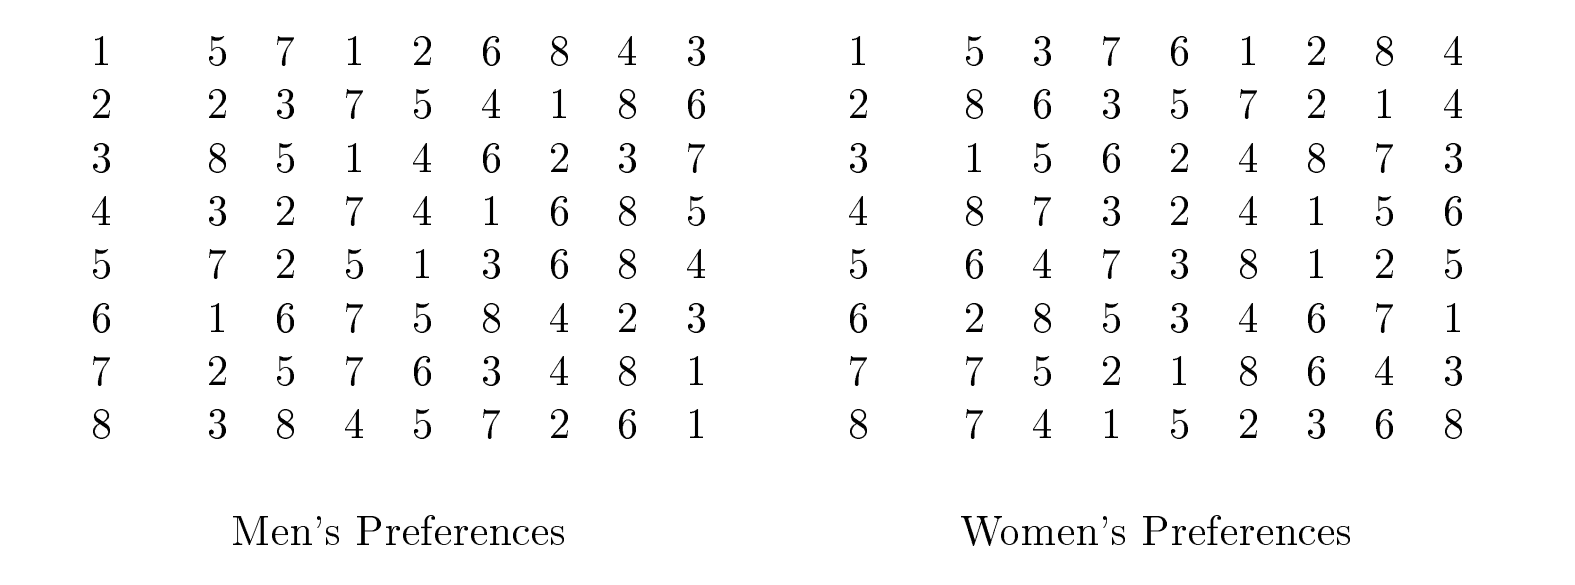
\includegraphics[width=1\textwidth]{IMAGES_FIGS/FIG_2_0.png}
  \caption{The stable marriage instance of size 8}
  \label{FIG_2_1}
\end{figure}

Let us consider the example of size eight. Here we have the lattice of 8 stable matchings for this instance. Each stable matching $M$ is described by a vector of length eight, where the number in position $i$ of the vector indicates the $M-partner$ of man $i$. Below each stable matching $M$ is a vector indicating the the ranking of the $M-partner$ of each man. 

\begin{figure}[ht]
  \centering
  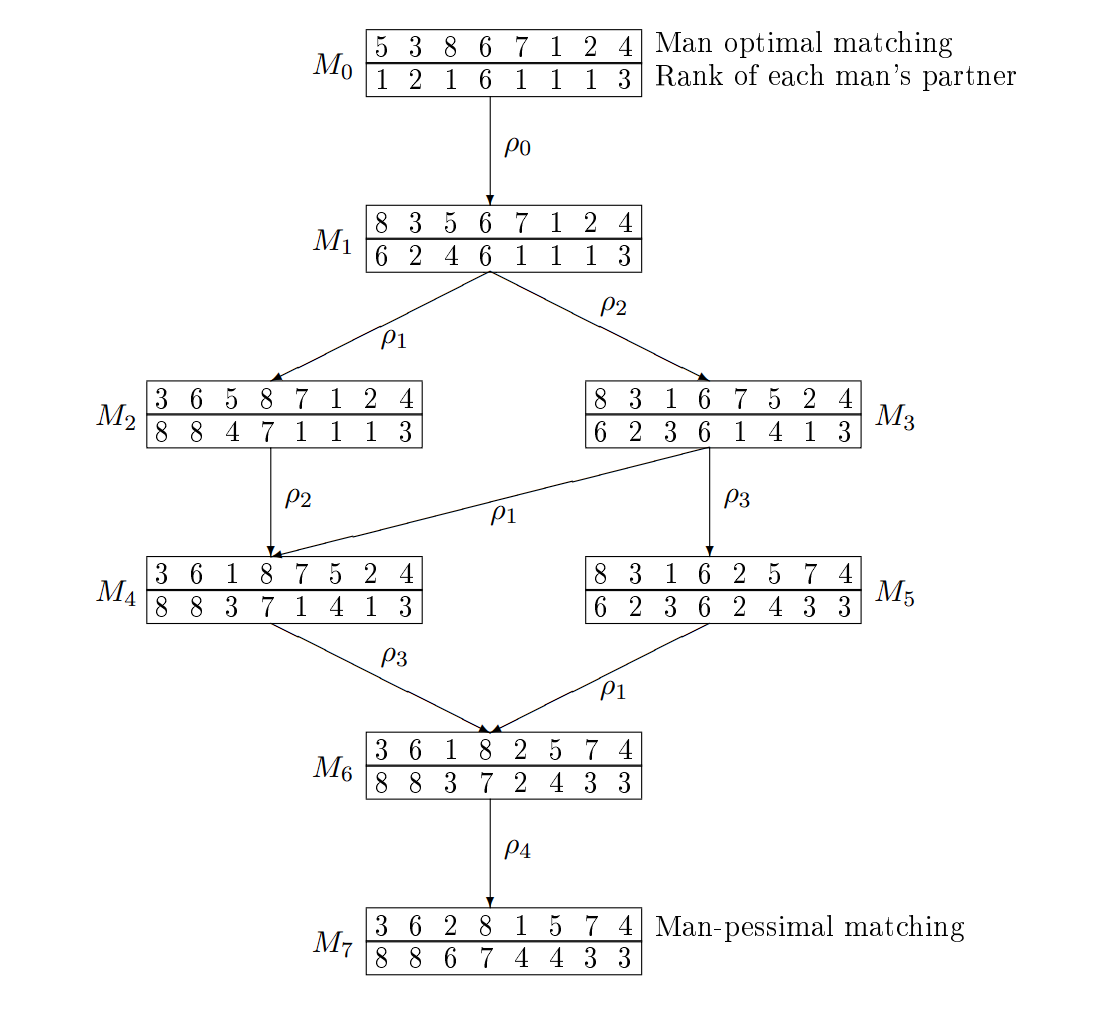
\includegraphics[width=0.9\textwidth]{IMAGES_FIGS/FIG_2_1.png}
  \caption{The lattice of stable matchings}
  \label{FIG_2_2}
\end{figure}

\begin{figure}[ht]
  \centering
  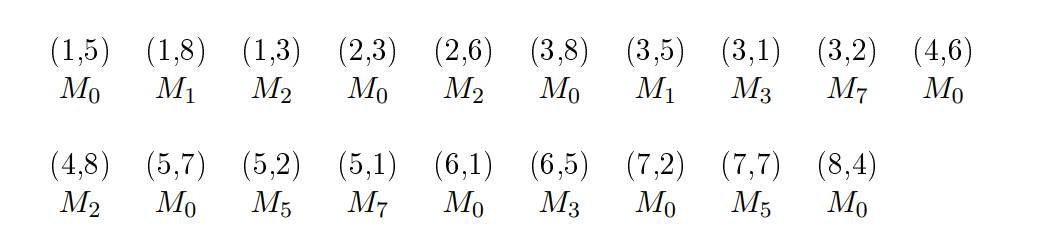
\includegraphics[width=0.8\textwidth]{IMAGES_FIGS/FIG_2_2.png}
  \caption{The stable pairs, and associated irreducible matchings}
  \label{FIG_2_3}
\end{figure}

\begin{figure}[ht]
  \centering
  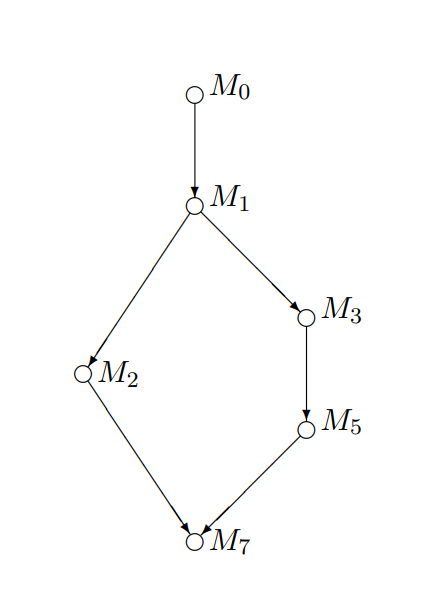
\includegraphics[width=0.4\textwidth]{IMAGES_FIGS/FIG_2_3.png}
  \caption{The partial order $I(\mathcal{M})$ for the irreducible stable matchings}
  \label{FIG_2_4}
\end{figure}

%make a box enclosing it
If $(R, \preceq)$ is a partial order, then a subset $S$ of $R$ is said to be \textbf{closed} in $R$ if there is no element in $R\backslash S$ that precedes an element in $S$.

A subset of matchings $S \subseteq M$ is closed in M if there is no matching in $M \\ S$ that dominates a matching in $S$.

Notice that, if $S$ is a subset of matchings in $I(\mathcal{M})$, then $\vee S$ is also a stable matching in $M$. Hence, every nonempty closed subset of $I(\mathcal{M})$ generates a stable matching in this way, and this defines a mapping from the nonempty closed subsets of $I(\mathcal{M})$ to $\mathcal{M}$. And we will show that this mapping is one-one.

For an arbitrary stable matching $M$, we define the irreducible support $U(M)$ of $M$ to be
$\{M(m, w) : (m, w) \in M\}$. 

\begin{exmp}\label{exmp_2_1}
    In the stable matchings of the above figure, the irreducible support of matching $M_3 = \{(1, 8),(2, 3),(3, 1),(4, 6),(5, 7),(6, 5),(7, 2),(8, 4)\}$ is $\{M_0, M_1, M_3\}$.
\end{exmp}

\begin{lemma}
\label{lem_2_1}
For any stable matching $M$, $M = \vee U(M)$.
\newline
\newline
\textit{{\small Any stable matching $M$ can be obtained by assigning each man to his least preferred partner among his partners in the matchings in $U(M)$}}
\end{lemma}

\begin{proof}
    Suppose $(m_1, w_1)$ is in $M$ but not in $\vee U(M)$. Since $(m_1, w_1)$ is in $M(m_1, w_1) \in U(M)$, there must be a pair $(m_2, w_2)$ in $M$ such that, in $M(m_2, w_2)$, man $m_1$ marries a woman strictly below $w_1$ in his list. Now $M(m_2, w_2)$ dominates all the stable matchings in which $m_2$ marries $w_2$, and in particular $M$. But this is a contradiction, because $m_1$ prefers $w_1$, his partner in $M$, to his partner in $M(m_2, w_2)$. Hence we have $M = \vee U(M)$.
\end{proof}

\begin{exmp}\label{exmp_2_2}
Woman $3$ is the worst partner for man $1$ among his partners in the matchings $\{M_0, M_2, M_3, M_5\} = U(M_6)$; woman $3$ is in fact the partner of man $1$ in $M_6$.
\end{exmp}

\begin{corollary}\label{cor_2_1}
Let $\hat{U}(M)$ be the set of all irreducible matchings that dominate some matching in $U(M)$. Then $M = \vee \hat{U}(M)$.
\end{corollary}

\begin{proof}
If a stable matching $M_1$ dominates stable matching $M_2$ then $M_1 \vee M_2 = M_2$, so $\vee \hat{U}(M) = \vee U(M)$, since each matching in $\hat{U}(M)$ dominates some matching in $U$.
\end{proof}

\begin{corollary}\label{cor_2_2}
A stable matching $M$ is $\vee S$ for a set $S$ of \textit{stable matchings} that excludes $M$, iff $M$ is not in $I(\mathcal{M})$
\end{corollary}

\begin{proof}
    The \textit{"if"} part follows from the Lemma studied earlier. Let's prove the converse part. First note that if $M = \vee S$, then every matching in $S$, dominates $M$. So if $M \notin S$, then for any pair $(m, w)$ in $M$ there is a matching $M^\prime$ in $S$ that contains $(m, w)$ and that strictly dominates $M$. So $M \neq M(m, w)$, and this is true for all pairs $(m, w)$ in $M$, so that $M$ cannot be in $I(\mathcal{M})$.
\end{proof}

Let's now prove that the mapping from the nonempty closed subsets of
$I(\mathcal{M})$ to $\mathcal{M}$ is one-one.

\begin{lemma}\label{lem_2_2}
    If $S$ and $T$ are \textit{distinct} closed subsets of $I(\mathcal{M})$, then $\vee S \neq \vee T$.
\end{lemma}

\begin{proof}
     Note, here that no maximal matching (with respect to dominance) of $S \cup T$ can dominate any other matching in $S \cup T$. Further, since $S \neq T$ and both subsets are closed in $I(\mathcal{M})$, one of the maximal matchings of $S \cup T$ cannot be in $S \cap T$. So one of the subsets, say $S$, contains a matching $M$ that does not dominate any matching in the other subset, $T$. Now $M = M(m, w)$ for some $m$ and $w$, so that $m$ has a partner no better than $w$ in $\vee S$. On the other hand, we claim that $m$ has a better partner than $w$ in every matching in $T$, so $\vee S$ cannot be $\vee T$. 
\end{proof}

\begin{theo}
So, in summary we have : 
\begin{itemize}
    \item There is a one-one correspondence between the nonempty closed subsets of $I(\mathcal{M})$ and the stable matchings of $\mathcal{M}$. This correspondence associates each stable matching $M$ with the irreducible stable matchings that dominates $M$.
    \item  If $S$ is the \textit{closed subset} of $I(\mathcal{M})$ corresponding to stable matching $M$, then $M = \vee S$.
    \item If closed subsets $S$ and $S^\prime$ of $I(\mathcal{M})$ correspond to matchings $M$ and $M^\prime$, respectively, then $M$ dominates $M^\prime$ \textbf{if and only if} $S \subseteq S^\prime$.
\end{itemize}

\end{theo}

\section{Generalizing to a ring of set}
Despite the possibility of constructing the partial order of irreducible matchings $I(\mathcal{M})$ in $\mathcal{O}(n^5)$ time, which facilitates the development of polynomial time algorithms for various problems related to stable marriage, these algorithms are not the most optimal known solutions for these problems.

In order to enhance computational efficiency, our approach involves the creation of a distinct, yet intimately related construct known as $\Pi(\mathcal{M})$, which can be generated from the preference lists within $\mathcal{O}(n^2)$ time. This newly proposed structure exhibits several valuable algorithmic properties that are not present in $I(\mathcal{M})$.

To facilitate the development of $\Pi(\mathcal{M})$, the initial step involves exploring the more comprehensive issue of effectively compacting the representation of a ring of sets. This entails creating a representation that is more general than $I(\mathcal{M})$, which will then be modified to form a related representation. We will discuss the construction of this representation and its efficiency in detail.

\subsection{Rings of Sets}

A \textbf{ring of sets} over a given set $B$, denoted by $\mathcal{F} = \{F_0 , \cdots \cdots, F_k\}$, is defined as a family of subsets of $B$ that satisfies the closure properties of \textit{set union} and \textit{intersection}. Specifically, if $F_i$ and $F_j$ are any two subsets of $B$ in $\mathcal{F}$, then $F_i \cup F_j$ and $F_i \cap F_j$ are also members of $\mathcal{F}$. Notably, since the members of $\mathcal{F}$ are subsets of $B$, if $S$ is a subset of $\mathcal{F}$, then $\cup \{F_i: F_i \in S\}$ is a set of elements of $B$ and thus belongs to $\mathcal{F}$.

Given that a ring of sets adheres to the closure properties of set \textit{union} and \textit{intersection}, it follows that there exist \textit{unique minimal} and \textit{maximal} elements within $\mathcal{F}$, determined in relation to set containment. In other words, the minimal element represents a subset of every other member of $\mathcal{F}$, while the maximal element represents a superset of every other member of $\mathcal{F}$.

\subsection{ The Stable Matchings Form a Ring of Sets}

It is plausible to consider the set of stable matchings $M$ for a given problem instance as a ring of sets. This can be demonstrated by presenting an alternate means of characterizing a stable matching.

Given a stable matching $M$, the set of all pairs $(m,w)$ where $w$ is either $p_M(m)$ (m's partner in M) or a woman whom $m$ prefers to $p_M(m)$ is referred to as the $P-set$ of $M$. We denote $P(M)$ as the $P-set$ of $M$, and $P(\mathcal{M})$ as the collection of $P-sets$ corresponding to the stable matchings of $\mathcal{M}$. It is noteworthy that a subset $P$ of the $n^2$ man-woman pairs is a P-set \textit{if and only if} $P = P(M)$ for some stable matching $M$.

It is important to observe that if $P$ corresponds to a $P-set$ of an unknown stable matching $M$, then $M$ can be explicitly derived from $P$ by matching each man $m$ with the woman $w$ he least prefers from the pairs $(m, w)$ in $P$.

%Add Figure ref here
\begin{exmp}\label{exmp_2_3}
    $M_0$ from Figure \ref{FIG_2_2} can be described as the $P-set$ \newline $\{(1, 5),(2, 2),(2, 3),(3, 8),(4, 3),(4, 2),(4, 7),(4, 4),(4, 1),(4, 6),(5, 7), \newline (6, 1),
(7, 2),(8, 3),(8, 8),(8, 4)\}$.
\end{exmp}

\begin{exmp}\label{exmp_2_4}
The $P-set$ for stable matching $M_3$ contains these pairs plus the pairs
$\{(1, 7),(1, 1),(1, 2),(1, 6),(1, 8),(3, 5),(3, 1),(6, 6),
(6, 7),(6, 5)\}$.
\end{exmp}

Given the above definitions, the following is now immediate.

\begin{lemma}\label{lem_2_3}
If $M$ and $M^\prime$ are two stable matchings, then $P(M \vee M^\prime) = P(M) \cup P(M^\prime)$ and $P(M \wedge M^\prime) = P(M) \cap P(M^\prime)$. 
\end{lemma}

It shows that $P(\mathcal{M})$ is a ring of sets for a marriage lattice $\mathcal{M}$. For a problem instance of size $n$, the \textit{base set} of the ring is the set of all $n^2$ man-woman pairs, and the family of $P-sets$, $P(\mathcal{M})$, is closed under set union and intersection. Since Stable matchings are closed under $\vee$ and $\wedge$.

Note that in $P(\mathcal{M})$ the man-optimal matching corresponds to the \textit{minimal} $P-set$, and the woman-optimal matching corresponds to the \textit{maximal} $P-set$.



\section{A Compact Representation of a Ring of Sets}

In this section, we demonstrate how the marriage lattice $\mathcal{M}$ representation, $I(\mathcal{M})$, can be extended to a general representation $I(\mathcal{F})$ for any ring of sets $\mathcal{F}$. The definitions and proofs in this section are very similar to those used for $I(\mathcal{M})$, although with some minor distinctions.

For any element $a \in B$, we let $\mathcal{F}(a)$ denote the set of all elements of $\mathcal{F}$ that contain $a$. It may happen that $\mathcal{F}(a)$ is empty, but if $F_i$ and $F_j$ belong to $\mathcal{F}(a)$, then so also do $F_i \cup F_j$ and $F_i \cap F_j$ . So $\mathcal{F}(a)$ itself forms a ring of sets over $B$, and there is therefore a \textbf{unique minimal} and a \textbf{unique maximal} element of $\mathcal{F}(a)$; we define $F(a)$ to be the unique \textit{minimal element} of $\mathcal{F}(a)$. That is, $F(a) = \{F : F \in \mathcal{F}(a)\}$. Then, an element $F$ of $\mathcal{F}$ that is $F(a)$ for some $a$ will be called $irreducible$, and we use $I(\mathcal{F})$ to denote the set of all \textit{irreducible elements} of $\mathcal{F}$. We also view $(I(F), \preceq)$ as a partial order under the relation $\preceq$ of set containment: if $F$ and $F^\prime$ are elements of $\mathcal{F}$, then $F$ precedes $F^\prime$ in $(I(F),\preceq)$ if and only if $F \subseteq F^\prime$.

\begin{exmp}\label{exmp_2_5}
 Consider the ring of sets $\mathcal{F}$ displayed by the \textit{Hasse diagram} of $\mathcal{F}$ in Figure \ref{FIG_2_5}. The base of this ring is the set $\{a, b, c, d, e, f, g, h, i\}$, and there is an edge from a set $F$ to a set $F^\prime$ if and only if $F$ is an immediate predecessor of $F^\prime$, i.e., $F \subset F^\prime$, and there is no set $F^{\prime \prime}$ such that $F \subset F^{\prime \prime} \subset F^\prime$. The \textit{irreducible} elements of the ring are $\{F_0, F_1, F_2, F_3, F_5, F_{11}\}$, and each such $F$ is $F(x)$ for every underlined element $x$ in $F$, i.e., $F$ is the minimal element of $\mathcal{F}$ containing $x \in B$. The partial order $I(\mathcal{F})$ is shown in Figure \ref{FIG_2_6}
\end{exmp}

\begin{figure}[ht]
  \centering
  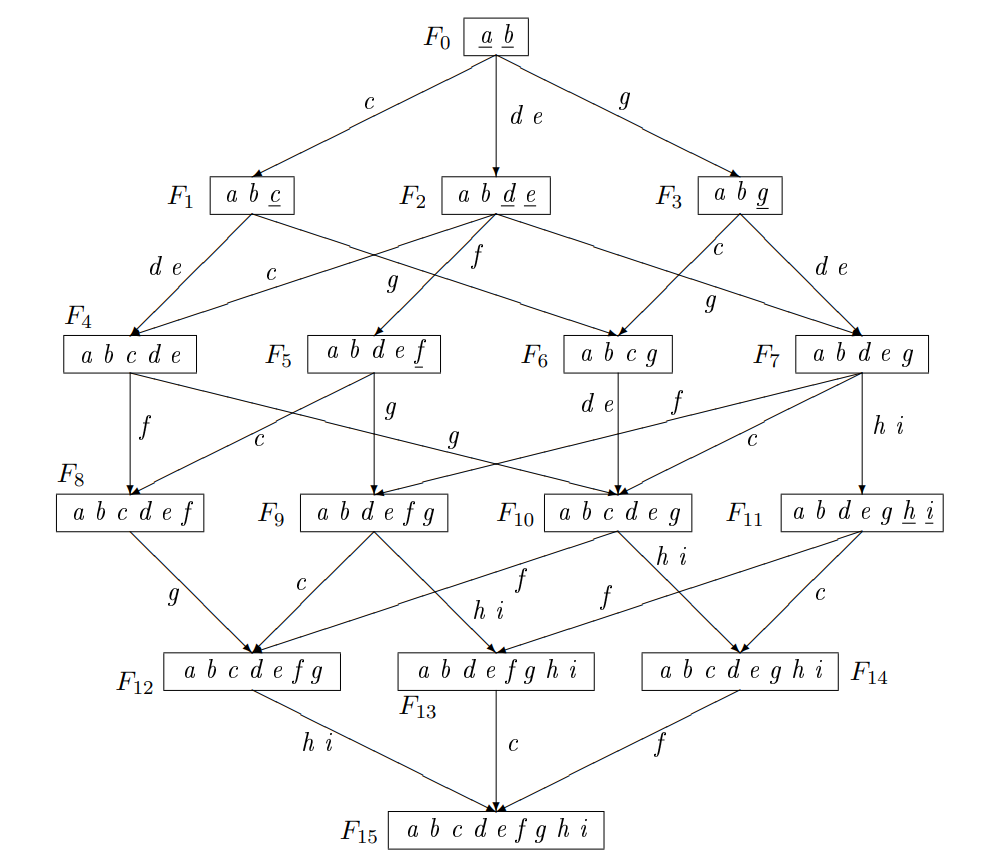
\includegraphics[width=1\textwidth]{IMAGES_FIGS/FIG_2_4.png}
  \caption{A ring of sets with $B = \{a, b, c, d, e, f, g, h, i\}$}
  \label{FIG_2_5}
\end{figure}

\begin{figure}[ht]
  \centering
  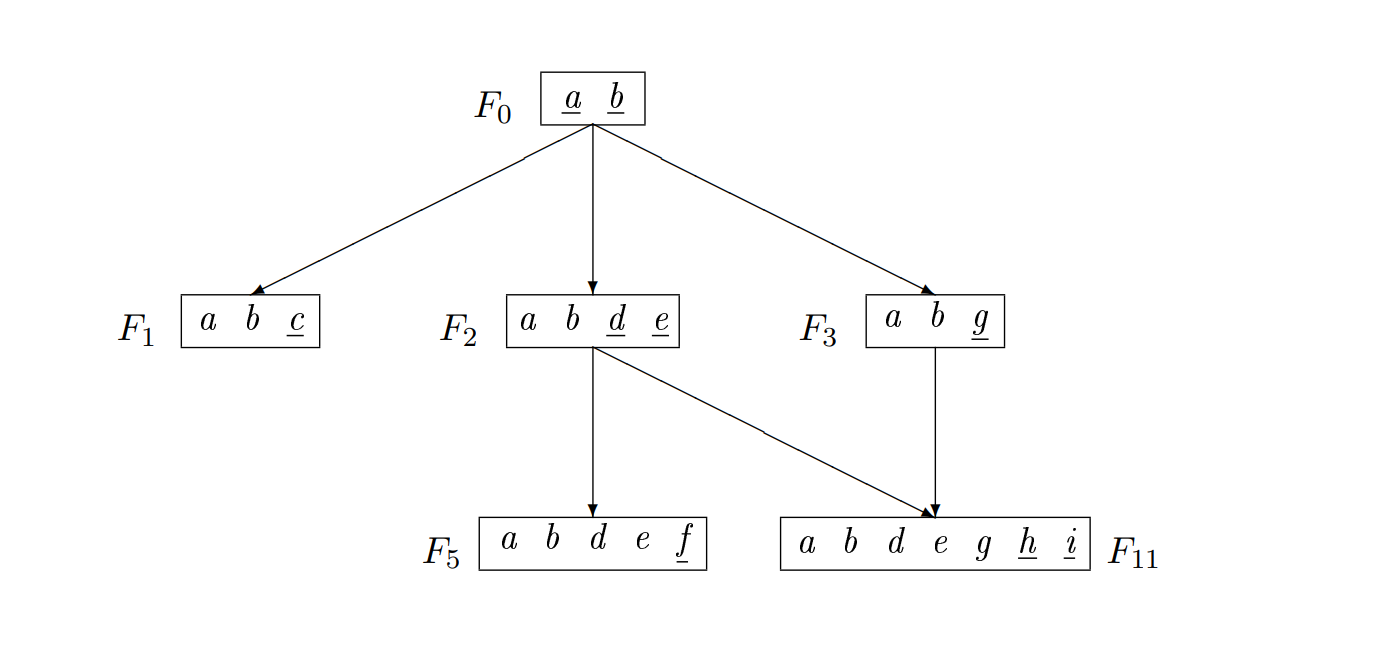
\includegraphics[width=0.85\textwidth]{IMAGES_FIGS/FIG_2_5.png}
  \caption{The partial order $I(\mathcal{F})$ of the irreducible elements of $\mathcal{F}$}
  \label{FIG_2_6}
\end{figure}

Let $S$ be any nonempty subset of $I(\mathcal{F})$. Since $\mathcal{F}$ is closed under \textit{union}, $\cup\{F : F \in S\}$ is a subset of B that is in $\mathcal{F}$. Hence each nonempty closed subset of $I(\mathcal{F})$ generates an element of $\mathcal{F}$ in this way. Our immediate objective is to show that this correspondence between nonempty closed subsets of $I(\mathcal{F})$ and elements of $\mathcal{F}$ is one-one.

For an arbitrary element $F$ of $\mathcal{F}$, we define the irreducible support $U(F)$ of $F$ to be $\{F(a): a \in$ $F\}$

\begin{lemma}\label{lem_2_4}
For any element $F$ of $\mathcal{F}$, the irreducible support of $F$ is closed in $I(\mathcal{F})$. Equivalently, $U(F)$ is the set of all irreducible elements of $\mathcal{F}$ that precede $F$ in $\mathcal{F}$, i.e., that are subsets of $F$.
\end{lemma}

\begin{proof}
Let $F_1 \subset F_2$ be two distinct irreducible elements of $\mathcal{F}$, and let $F_2$ be in $U(F)$. We will show that $F_1$ is in $U(F)$. Since $F_1$ is irreducible, $F_1=F(b)$ for some $b \in B$. Similarly, $F_2=F(a)$ for some $a \in F$, so $b$ must be in $F(a)$. Now $a \in F$ implies that $F(a) \subseteq F$, so it follows that $b$ is in $F$, and hence $F(b)$, which is $F_1$, is in $U(F)$.
\end{proof}

\begin{exmp}\label{exmp_2_6}
    We have $U\left(F_9\right)=\left\{F_0, F_2, F_3, F_5\right\}$, which is indeed closed in $I(\mathcal{F})$, and is the set of all irreducible elements of $\mathcal{F}$ that precede $F_9$ in $\mathcal{F}$. Note that we have not defined any object similar to $\hat{U}$, the closure of $U$, which was defined in the discussion of $I(\mathcal{M})$. The reason is that, unlike $U(F)$, which is closed in $\mathcal{F}, U(M)$ is not always closed for any $M \in \mathcal{M}$.
\end{exmp}

\begin{lemma}\label{lem_2_5}
 For any element $F$ of $\mathcal{F}, F=\cup U(F)$. That is, $F$ can be expressed as the union of its irreducible support.   
\end{lemma}

\begin{proof}
    For any element $a \in F, a$ is in $F(a)$, which is in $U(F)$, so $a$ is in $\cup U(F)$, hence $F \subseteq \cup U(F)$. Conversely, every element of $U(F)$ is a subset of $F$, so $\cup U(F) \subseteq F$.
\end{proof}

\begin{lemma}\label{lem_2_6}
    $F$ is irreducible if and only if $F$ cannot be written as the union of members of $\mathcal{F}$ excluding $F$ itself.
\end{lemma}

\begin{lemma}\label{lem_2_7}
    If $S$ and $T$ are distinct closed subsets of $I(\mathcal{F})$, then $\cup S \neq \cup T$.
\end{lemma}

\begin{proof}
    If $S$ and $T$ are different closed subsets of $I(\mathcal{F})$, then one of them, say $S$, contains an element $F=F(a)$ that is not contained in the other set, $T$. But $F(a)$ is contained in all members of $\mathcal{F}$ that contain $a$, so no such member of $\mathcal{F}$ is in $T$. Hence $a \in \cup S, a \notin \cup T$, and therefore $\cup S \neq \cup T$.
\end{proof}
\newpage
\begin{theo}
So, in summary we have :
\begin{itemize}
    \item There is a one-one correspondence between the elements of $\mathcal{F}$ and the nonempty closed subsets of $I(\mathcal{F})$. In particular, an element $F$ of $\mathcal{F}$ corresponds to $U(F)$, which is a closed subset in $I(\mathcal{F})$.
    \item Each nonempty closed subset of $I(\mathcal{F})$ generates (by unioning) an element of $\mathcal{F}$, and each element of $\mathcal{F}$ is generated in this way by exactly one nonempty closed subset of $I(\mathcal{F})$.
    \item If $S$ and $S^{\prime}$ are closed subsets of $I(\mathcal{F})$ that generate $F$ and $F^{\prime}$ respectively, then $F \subseteq F^{\prime}$ if and only if $S \subseteq S^{\prime}$.
\end{itemize}
\end{theo}

\begin{exmp}\label{exmp_2_7}
    There are sixteen nonempty closed subsets of $I(\mathcal{F})$ each generates a distinct element of $\mathcal{F}$, and each is the irreducible support of that element. Figure \ref{FIG_2_7} shows the elements of $\mathcal{F}$, and for each one, the unique nonempty closed subset of $I(\mathcal{F})$ that generates it.
\end{exmp}

\begin{center}
    $\begin{array}{lllllll}F_0: & F_0 & & & & & \\ F_1: & F_0 & F_1 & & & & \\ F_2: & F_0 & F_2 & & & & \\ F_3: & F_0 & F_3 & & & & \\ F_4: & F_0 & F_1 & F_2 & & & \\ F_5: & F_0 & F_2 & F_5 & & & \\ F_6: & F_0 & F_1 & F_3 & & & \\ F_7: & F_0 & F_2 & F_3 & & & \\ F_8: & F_0 & F_1 & F_2 & F_5 & & \\ F_9: & F_0 & F_2 & F_3 & F_5 & & \\ F_{10}: & F_0 & F_1 & F_2 & F_3 & & \\ F_{11}: & F_0 & F_2 & F_3 & F_{11} & & \\ F_{12}: & F_0 & F_1 & F_2 & F_3 & F_5 & \\ F_{13}: & F_0 & F_2 & F_3 & F_5 & F_{11} & \\ F_{14}: & F_0 & F_1 & F_2 & F_3 & F_{11} & \\ F_{15}: & F_0 & F_1 & F_2 & F_3 & F_5 & F_{11} \end{array}$
    \begin{figure}[ht]
  \centering
  \caption{The elements of $\mathcal{F}$ and their associated closed subsets of $I(\mathcal{F})$}
  \label{FIG_2_7}
\end{figure}
    %REF TO FIGURE
\end{center}

\subsection{$I(\mathcal{F})$ reduces to $I(\mathcal{M})$}
When $\mathcal{F}$ is $P(\mathcal{M})$, the ring of $P$-sets corresponding to the stable matchings in $\mathcal{M}$, then the partial order $I(\mathcal{F})$ specializes to the partial order $I(\mathcal{M})$ defined in the previous section. Note however that not all of the ring definitions specialize directly to matching definitions. In particular, if $a=(m, w)$, then $\mathcal{F}(a)$ is the set of all $P$-sets containing the pair $(m, w)$, i.e., $\mathcal{F}(a)$ is the set of all stable matchings where $m$ marries $w$ or a woman below $w$ in his list. Hence $\mathcal{F}(a)$ is not $\mathcal{M}(m, w)$, since $\mathcal{M}(m, w)$ is the set of stable matchings in which $m$ marries $w$. Similarly, $U(P(M))$ contains the $P$-sets of all the matchings of $\hat{U}(M)$, rather than just those of $U(M)$. However, $F(a)$ is equal to $M(m, w)$, and this is enough to imply that when $\mathcal{F}$ is $P(\mathcal{M})$, the partial order $I(\mathcal{F})$ specializes to the partial order $I(\mathcal{M})$ defined for $\mathcal{M}$.


\section{Representing a Ring of Sets by Set Differences}

In this section we continue our examination of a general ring of sets $\mathcal{F}$, focusing on the set differences between elements of $\mathcal{F}$. We will then use certain set differences to define a new representation of $\mathcal{F}, D(\mathcal{F})$, that will be more useful than $I(\mathcal{F})$ for algorithmic purposes, and in the case of the stable marriage problem, can be more efficiently constructed than $I(\mathcal{M})$.

\subsection{The Centers of a Ring of Sets}

The unique minimal element of a ring of sets $\mathcal{F}$ will be called the zero of $\mathcal{F}$, and will be denoted by $F_0$. For an irreducible element $F$ of $\mathcal{F}$, the center of $F$, written $K(F)$, is the set $\{a \in B: F(a)=F\}$. Note that the center of an element $F$ is defined only if $F$ is irreducible. Note also that $K\left(F_0\right)=F_0$. but for any other irreducible element $F, K(F) \subset F$, since $F_0 \subset F$. In each irreducible element $F$ of $\mathcal{F}$, shown in Figures \ref{FIG_2_5} and \ref{FIG_2_6} , the elements of $B$ in the center of $F$ are underlined. So, for example, the center of $F_2$ is $\{d, e\}$.

\begin{lemma}\label{lem_2_8}
 Every element of $B$ is a member of at most one center of $\mathcal{F}$.
\end{lemma}

\begin{proof}
    If $a \in K\left(F_i\right) \cap K\left(F_j\right)$, then $F_i=F(a)=F_j$.
\end{proof}

\subsection{The centers represent a ring of sets}
 
 Just as every element $F \in \mathcal{F}$ can be expressed as the union of the irreducible elements that precede it in $\mathcal{F}, F$ can also be expressed as the union of the centers of the irreducible elements that precede $F$ in $\mathcal{F}$. This provides a more revealing and economical expression for $F$, since distinct centers never intersect. 
\begin{lemma}\label{lem_2_9}
    For any element $F$ in $\mathcal{F}, F=\bigcup\left\{K\left(F_i\right): F_i \in U(F)\right\}$. Further, this is the only way to express $F$ as the union of a set of centers of $\mathcal{F}$.
\end{lemma}

\begin{proof}
     By definition of $U(f), F(a)$ is in $U(F)$ for every $a$ in $F$. Also, $a$ must be in $K(F(a))$, which is a subset of $F(a)$. It follows then that $F \subseteq \bigcup\left\{K\left(F_i\right): F_i \in U(F)\right\}$. Conversely, for every $F(a) \in U(F), F(a)$ is a subset of $F$, so $K(F(a))$ is a subset of $F$, and hence $\left\{K\left(F_i\right)\right.$ : $\left.F_i \in U(F)\right\} \subseteq F$. The uniqueness of the expression follows from the fact that no distinct centers intersect.
\end{proof}

We now define $D(\mathcal{F})$ to be the set of all centers of $\mathcal{F}$ other than $F_0$. The set $D(\mathcal{F})$ will allow us to focus on and characterize the minimal differences between elements of $\mathcal{F}$. These differences will serve as building blocks to construct and represent $\mathcal{F}$. We begin to make this precise with the following immediate corollaries of Lemma \ref{lem_2_9}.


\begin{corollary}\label{cor_2_3}
For any distinct elements $F_i$ and $F_j$ in $\mathcal{F}$, the symmetric difference of $F_i$ and $F_j,\left(F_i \backslash F_j\right) \cup\left(F_j \backslash F_i\right)$, is the union of a set of centers in $D(\mathcal{F})$. Further, there is only one set of centers whose union is the symmetric difference of $F_i$ and $F_j$.
\end{corollary}

\begin{exmp}\label{exmp_2_8}
    The symmetric difference of $F_8$ and $F_{11}$ shown in Figure \ref{FIG_2_5} is $\{c, f, g, h, i\}$, which is the union of $\left\{K\left(F_1\right), K\left(F_3\right), K\left(F_5\right), K\left(F_{11}\right)\right\}$, as may easily be verified.
\end{exmp}

\begin{corollary}\label{cor_2_4}
    If $F_0$ and $F_z$ are respectively the minimal and maximal elements of $\mathcal{F}$, then $F_z \backslash F_0$ is the union of all the centers in $D(\mathcal{F})$. i.e., $F_z \backslash F_0=\bigcup\left\{K\left(F_i\right): F_i \in I(\mathcal{F}) \backslash F_0\right\}$.
\end{corollary}

The following Lemma is a partial converse to Corollary \ref{cor_2_3}.

\begin{lemma}\label{lem_2_10}
    Every center $K(F)$ in $D(\mathcal{F})$ is the symmetric difference of a pair of elements of $\mathcal{F}$. In fact, $K(F)=F \backslash \hat{F}$, where $\hat{F} \subset F$ is an element of $\mathcal{F}$.
\end{lemma}

\begin{proof}
    Let $F$ be any nonzero element of $I(\mathcal{F})$, and let $\hat{F}$ be the union of all elements of $\mathcal{F}$ that strictly precede $F$. Clearly, $\hat{F}$ is an element of $\mathcal{F}$, and $\hat{F} \subset F$, so $F \backslash \hat{F}$ is a symmetric difference of a pair of elements of $\mathcal{F}$. Further, it follows easily from the definition of $K(F)$ that $F \backslash \hat{F} \subseteq K(F)$, and $K(F) \subseteq F \backslash \hat{F}$, so $F \backslash \hat{F}=K(F)$.
\end{proof}

\subsection{The minimal differences of $\mathcal{F}$}


Lemma \ref{lem_2_10} and Corollary \ref{cor_2_3} establish that the elements of $D(\mathcal{F})$ are precisely the minimal elements, with respect to set containment, of the set of all symmetric differences of distinct elements in $\mathcal{F}$. That is, every symmetric difference of a pair of elements in $\mathcal{F}$ is the union of a set of centers in $D(\mathcal{F})$, and every element in $D(\mathcal{F})$ is the symmetric difference of a pair of elements of $\mathcal{F}$. This view of $D(\mathcal{F})$ will be essential, and in order to emphasize the connection of $D(\mathcal{F})$ to set differences, we will hereafter refer to a center of $F \in D(\mathcal{F})$ as a minimal difference of $F$ and use the notation $D(F)$ in place of $K(F)$. The set $D(\mathcal{F})$ will be called the set of minimal differences of $\mathcal{F}$.

\subsection{The Partial Order of Minimal Differences}
Given the close connection between the sets $D(\mathcal{F})$ and $I(\mathcal{F})$, and the fact that the nonempty closed subsets of $I(\mathcal{F})$ represent $\mathcal{F}$, it should not be surprising that the closed subsets of $D(\mathcal{F})$ can also be used to represent $\mathcal{F}$ as we now show.

We define $(D(\mathcal{F}), \preceq)$ to be the partial order on the set $D(\mathcal{F})$ obtained by removing $F_0$ from the partial order $I(\mathcal{F})$ and then replacing each remaining element $F \in I(\mathcal{F})$ by its associated minimal difference $D(F)$. The precedence relation $(\preceq)$ on $D(\mathcal{F})$ is inherited from the precedence relation on $I(\mathcal{F})$ (and hence from $\mathcal{F}$): $D(F)$ precedes $D\left(F^{\prime}\right)$ in $(D(\mathcal{F}) \preceq)$ if and only if $F$ precedes $F^{\prime}$ in $I(\mathcal{F})$, i.e., $F \subseteq F^{\prime}$. In other words, the partial order $D(\mathcal{F})$ is isomorphic to the partial order $I(\mathcal{F})$ after the removal of the unique minimal element from $I(\mathcal{F})$. Figure \ref{FIG_2_8} shows the representation $D(\mathcal{F})$ obtained from $I(\mathcal{F})$ of Figure \ref{FIG_2_6}.

Now each minimal difference is associated with exactly one element of $I(\mathcal{F})$, and the precedence relation on $D(\mathcal{F})$ agrees with the relation on $I(\mathcal{F})$, so there is a one-one correspondence between the non-empty closed subsets of $I(\mathcal{F})$ and the closed subsets (including the empty subset) of $D(\mathcal{F})$; the closed subset of $I(\mathcal{F})$ consisting of $F_0$ corresponds to the empty subset of $D(\mathcal{F})$. Given the one-one correspondence between the elements of $\mathcal{F}$ and the nonempty closed subsets of $I(\mathcal{F})$ , the following is immediate.
%\newline
%\pagebreak

\begin{theo}
There is a one-one correspondence between the elements of $\mathcal{F}$ and the closed subsets of $D(\mathcal{F})$. Further, if $F_i$ and $F_j$ are elements in $\mathcal{F}$ corresponding to closed subsets $D_i$ and $D_j$ of $D(\mathcal{F})$, then $F_i \subset F_j$ if and only if $D_i \subset D_j$
\end{theo}

\begin{figure}[h]
  \centering
  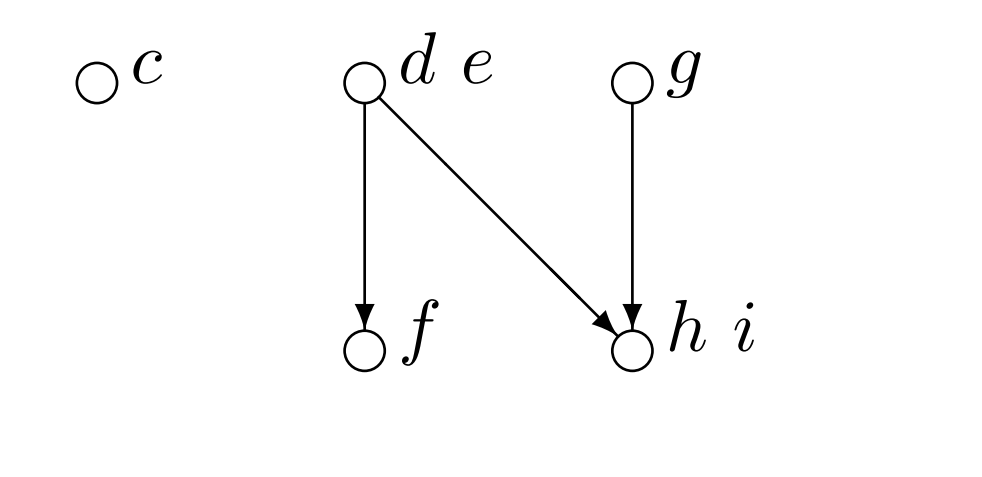
\includegraphics[width=0.5\textwidth]{IMAGES_FIGS/FIG_2_6.png}
  \caption{The partial order $D(\mathcal{F})$ for $\mathcal{F}$}
  \label{FIG_2_8}
\end{figure}

\section{Minimal Differences and Chains}

The partial order $D(\mathcal{F})$ provides a compact representation of $\mathcal{F}$, but its elements, the minimal differences of $\mathcal{F}$, are defined from the (generally hard to obtain) irreducible elements of $\mathcal{F}$, or worse, by the (huge) set of symmetric differences of elements of $\mathcal{F}$. Hence, we have no indication so far that minimal differences are easy to find, although we know there are at most $|B|$ of them, since by Lemma \ref{lem_2_8} , no element of $B$ is in more than one minimal difference. In this section we show that the minimal differences show up repeatedly and in a predictable way in $\mathcal{F}$, and this will be the key to efficiently finding them in $P(\mathcal{M})$. 

\begin{exmp}\label{exmp_2_9}
Consider again the Hasse diagram in Figure \ref{FIG_2_5} . On each edge connecting an element $F^{\prime}$ with its immediate predecessor $F$, we have shown the set $F^{\prime} \backslash F$. The interesting point to note is that each of these differences is a minimal difference of $\mathcal{F}$. In this section we will prove that this is true for any ring of sets; this will make it possible to identify the minimal differences of a ring of sets without knowing its irreducible elements, and that will be crucial in efficiently building $\Pi(\mathcal{M})$, our desired representation of $\mathcal{M}$.
\end{exmp}

A chain $C=\left\{C_1, \ldots, C_q\right\}$ in $\mathcal{F}$ is an ordered set of elements of $\mathcal{F}$ such that $C_i$ is an immediate predecessor of $C_{i+1}$, for each $i \leq i \leq q-1$. An $F_0$-chain is a chain that extends from the minimal element of $\mathcal{F}, F_0$, and a maximal $F_0$-chain, or maximal chain for short, is a chain that extends from $F_0$ to the maximal element $F_z$ of $\mathcal{F}$.

\begin{lemma}\label{lem_2_11}
Let $F$ and $F^{\prime}$ be any elements of $\mathcal{F}$ (not necessarily irreducible), and suppose $F$ is an immediate predecessor of $F^{\prime}$ in $\mathcal{F}$. Then $F^{\prime} \backslash F$ is a minimal difference of $\mathcal{F}$, that is, it is an element of $D(\mathcal{F})$.
\end{lemma}


 \begin{proof}
 Suppose $F^{\prime} \backslash F=D$, and let $\bar{F}$ be a minimal element of $\mathcal{F}$ that contains $D$. It is then immediate that $\bar{F} \subseteq F^{\prime}$, that $\bar{F} \cup F=F^{\prime}$, and that $\bar{F} \nsubseteq F$, so $\bar{F} \neq F_0$. Now if $F(a)$ is not $\bar{F}$ for some given element $a \in D$, then $F(a) \subset \bar{F}$, and $F \subset(F \cup F(a)) \subset(F \cup \bar{F})=F^{\prime}$, contradicting the assumption that $F$ is an immediate predecessor of $F^{\prime}$. Hence $F(a)=\bar{F}$ for every $a \in D$, so $\bar{F}$ is an irreducible element of $\mathcal{F}$, and $D \subseteq D(\bar{F})$. Now if $D \subset D(\bar{F})$, then $F^{\prime}=(F \cup D) \subset(F \cup D(\bar{F})) \subseteq(F \cup \bar{F})=F^{\prime}$, an impossibility. Hence $D=D(\bar{F})$, and so $D$ is a minimal difference of $\mathcal{F}$.
\end{proof}

If $D$ is the difference between two consecutive elements on a chain $C$ in $\mathcal{F}$, then we say that that $C$ \textit{contains} the difference $D$, and $D$ \textit{appears} on $C$. Note that by 2.4.4, $D$ is a minimal difference of $\mathcal{F}$. The following theorem is another reflection of the way that the structure of $\mathcal{F}$ is determined and expressed by its minimal differences.

\begin{theorem}\label{thm_2_1}
If $F^{\prime}$ and $F$ are any two elements in $\mathcal{F}$ such that $F$ precedes $F^{\prime}$, then every chain from $F$ to $F^{\prime}$ in $\mathcal{F}$ contains exactly the same set of minimal differences, although in a different order. In particular, if $F=F_0$, then every $F_0$-chain ending at $F^{\prime}$ contains the same set of minimal differences.
\end{theorem}

\begin{proof}
    Let $C$ be a chain that leads from $F$ to $F^{\prime}$. Clearly, $F^{\prime} \backslash F$ is the union of the consecutive (minimal) differences along $C$. But by Corollary \ref{cor_2_3}, this set of minimal differences must be unique, and the theorem follows.
\end{proof}

\begin{corollary}\label{cor_2_5}
If $C$ is any maximal chain in $\mathcal{F}$, then each difference of consecutive elements on $C$ is a minimal difference of $\mathcal{F}$, and each minimal difference of $\mathcal{F}$ appears exactly once as a difference of consecutive elements on $C$.
\end{corollary}

\begin{corollary}\label{cor_2_6}
    Every maximal chain in $\mathcal{F}$ has exactly $|D(\mathcal{F})|+1$ elements.
\end{corollary}

Corollary \ref{cor_2_5} will be the key to efficiently finding the minimal differences of $P(\mathcal{M})$, without needing to know in advance the matchings in $I(\mathcal{M})$.

Theorem \ref{thm_2_1} and its corollaries are very clearly illustrated in Figure \ref{FIG_2_5}. For example, there are three chains from $F_2$ to $F_{13}$. Each contains the minimal differences $\{f\},\{g\}$, and $\{h, i\}$, but in a different order on each chain. 

\subsection{Relating Chains to Closed Subsets}

Theorem \ref{thm_2_1} establishes a one-one correspondence between the elements of $\mathcal{F}$ and certain subsets of $D(\mathcal{F})$. However, established a one-one correspondence result between the elements of $\mathcal{F}$, and the closed subsets of $D(\mathcal{F})$. How these two correspondences relate to each other ? The answer is that they are identical.

\begin{theorem}\label{thm_2_2}
    The set of minimal differences along any $F_0$-chain $C$ is a closed subset of $D(\mathcal{F})$. Conversely, if $S$ is a closed subset of $D(\mathcal{F})$ corresponding to element $F \in \mathcal{F}$, then the $F_0$-chain in $\mathcal{F}$ ending at $F$ contains exactly the elements of $S$.
\end{theorem}

\begin{proof}
    Let $C$ end with element $F \in \mathcal{F}$. Clearly, $F$ is the union of $F_0$ and the differences of consecutive elements on $C$. Now by Corollary \ref{cor_2_5} , each of these consecutive differences is a minimal difference of $\mathcal{F}$, so $F$ is the union of $F_0$ and a set of minimal differences of $\mathcal{F}$. But by Lemma \ref{lem_2_9}, $F$ can be expressed in only one such way, and so by correspondence result the minimal differences on $C$ must be the minimal differences in the closed subset of $D(\mathcal{F})$ that generates $F$. Conversely, if $S$ is a closed subset of $D(\mathcal{F})$ corresponding to element $F \in \mathcal{F}$, and $C$ is any chain in $\mathcal{F}$ ending at $F$, then $F$ equals $F_0$ unioned with the minimal differences in $S$, and also equals $F_0$ unioned with the minimal differences along $C$. Then by Lemma \ref{lem_2_9}, these sets of minimal differences must be the same.
\end{proof}

\begin{exmp}\label{exmp_2_10}
In Figure \ref{FIG_2_5} every chain from $F_0$ to $F_9$ contains the minimal differences $\{d, e\},\{g\}$, and $\{f\}$, and these minimal differences indeed form the closed subset of $D(\mathcal{F})$ that corresponds to $F_9$.
\end{exmp}

With Theorem \ref{thm_2_2} we can now establish a direct connection between the precedence relation on $D(\mathcal{F})$ and the order that the minimal differences appear on chains in $\mathcal{F}$. This relationship will be one of the keys to efficiently deducing the precedence relation on $D(\mathcal{M})$, even when the associated matchings in $I(\mathcal{M})$ are unknown.

\begin{theorem}\label{thm_2_3}
    Let $F_i$ and $F_j$ be two nonzero irreducible elements of $\mathcal{F}$. Then $D\left(F_i\right)$ precedes $D\left(F_j\right)$ in $D(\mathcal{F})$ if and only if $D\left(F_i\right)$ appears before $D\left(F_j\right)$ on every maximal chain in $\mathcal{F}$.
\end{theorem}

\begin{proof}
    Suppose $D\left(F_i\right)$ appears before $D\left(F_j\right)$ on every maximal chain in $\mathcal{F}$. Then by Theorem \ref{thm_2_2}, $D\left(F_i\right)$ is in every closed subset of $D(\mathcal{F})$ that contains $D\left(F_j\right)$, and in particular, the closed subset consisting of all the predecessors of $D\left(F_j\right)$. Hence $D\left(F_i\right)$ does precede $D\left(F_j\right)$ in $D(\mathcal{F})$.

    Conversely, suppose that $D\left(F_i\right)$ precedes $D\left(F_j\right)$ in $D(\mathcal{F})$, and hence any closed subset of $D(\mathcal{F})$ containing $D\left(F_j\right)$ also contains $D\left(F_i\right)$. Now suppose there is an $F_0$-chain $C$ in which $D\left(F_i\right)$ appears before $D\left(F_j\right)$, and let $S$ be the set of minimal differences on $C$ ending with $D\left(F_i\right)$. Then by Theorem \ref{thm_2_2}, $S$ is a closed subset of $D(\mathcal{F})$ that contains $F_i$ but not $F_j$, a contradiction.
\end{proof}

\begin{exmp}\label{exmp_2_11}
    Consider the minimal differences $\{d, e\},\{c\}$, and $\{h, i\}$ in the partial order $D(\mathcal{F})$ of Figure \ref{FIG_2_8} . The minimal difference $\{d, e\}$ precedes $\{h, i\}$ in $D(\mathcal{F})$ and, as shown in Figure \ref{FIG_2_5},$\{d, e\}$ appears before $\{h, i\}$ on every maximal chain in $\mathcal{F}$. Also in that figure, there are chains in which $\{c\}$ appears before $\{d, e\}$, and chains where it appears after $\{d, e\}$; as required by Theorem \ref{thm_2_3}, these two minimal differences are incomparable in $D(\mathcal{F})$.
\end{exmp}



\chapter{Rotations}

\section{Introduction}
Let $M$ be a stable matching. For any man $m$ let $s_M(m)$ denote the first woman $w$ on $m$ 's list such that $w$ strictly prefers $m$ to $p_M(w)$ (her partner in $M$ ). Let next $_M(m)$ denote the partner in $M$ of woman $s_M(m)$. Note that since $M$ is stable, $m$ prefers $p_M(m)$ to $s_M(m)$. Note also that $s_M(m)$ might not exist. For example, if $M$ is the woman optimal matching, then $s_M(m)$ does not exist for any man.

\begin{exmp}\label{exmp_3_1}
Consider the stable matching $M_1$ from Figure \ref{FIG_2_2}. 

\begin{center}
    $\begin{array}{lll}1: & 3 & 2 \\ 2: & 8 & 1 \\ 3: & 1 & 6 \\ 4: & 8 & 1 \\ 5: & 2 & 7 \\ 6: & 5 & 3 \\ 7: & 5 & 3 \\ 8: & 2 & 7\end{array}$

    \begin{figure}[ht]
  \centering
  \caption{Woman $s_{M_1}(m)$ and man $\operatorname{next}_{M_1}(m)$ for each man $m$}
  \label{FIG_3_1}
\end{figure}
\end{center}
\end{exmp}

There is another way to think about $s_M(m)$ and $\operatorname{next}_M(m)$ that is motivated by the extended version of the Gale-Shapley algorithm discussed earlier. Suppose for each woman $w$ we delete all pairs $\left(m^{\prime}, w\right)$ such that $w$ prefers $p_M(w)$ to $m^{\prime}$. It is easy to see that in the resulting lists, which we call reduced lists, $p_M(w)$ is the last entry in $w$'s list, and $s_M(m)$ is the entry just following $p_M(m)$ in $m$ 's list. It is also true that $p_M(m)$ is the first entry in $m$'s list (hence $s_M(m)$ is the second entry), for if any woman $w^{\prime}$ remains above $p_M(m)$ after the deletions, then $w^{\prime}$ prefers $m$ to her partner in $M$, and $\left(m, w^{\prime}\right)$ would block $M$. So, after the deletions, $p_M(m)$, $s_M(m)$, and $p_M(w)$ are easy to identify, and $\operatorname{next}_M(m)$ is also easy to find, since it is the last entry on $p_M(m)$ 's new list; equivalently, $\operatorname{next}_M(m)$ is the man $m^{\prime}$ such that $p_M(m)$ is the first entry on the reduced list of $m^{\prime}$.

Note that when $M=M_0$, the reduced lists are the MGS-lists defined and discussed in the previous chapter. The use of reduced lists will streamline the presentation of certain algorithms to be discussed later.

\begin{center}
    $\begin{array}{llllll}
    1: & 8 & 3 & & & \\ 2: & 3 & 6 & & & \\ 3: & 5 & 1 & 6 & 2 & \\ 4: & 6 & 8 & 5 & & \\ 5: & 7 & 2 & 1 & 3 & 6 \\ 6: & 1 & 5 & 2 & 3 &  \\ 7: & 2 & 5 & 7 & 8 & 1 \\ 8: & 4 & 2 & 6 & &\end{array}$
    \begin{figure}[ht]
  \centering
  \caption{The reduced lists of the men for stable matching $M_1$}
  \label{FIG_3_2}
\end{figure}
\end{center}

 As an example, Figure \ref{FIG_3_2} shows the reduced lists of the men when $M$ is the stable matching $M_1$ of Figure \ref{FIG_2_2}.

Let $\rho=\left(m_0, w_0\right),\left(m_1, w_1\right), \ldots,\left(m_{r-1}, w_{r-1}\right)$ be an ordered list of pairs in a stable matching $M$ such that for each $i(0 \leq i \leq r-1), m_{i+1}$ is $\operatorname{next}_M\left(m_i\right)$, where $i+1$ is taken modulo $r$. Then $\rho$ is called a rotation (exposed) in $M$, and we say that $m$ (or $w$ ) is in rotation $\rho$ if there is a pair $(m, w)$ in the ordered list defining $\rho$. From this point on, it will be assumed that whenever we refer to an element $m_i$ or $w_i$ in a rotation $\left(m_0, w_0\right),\left(m_1, w_1\right), \ldots,\left(m_{r-1}, w_{r-1}\right)$, the value of the subscript $i$ is taken modulo $r$.

\begin{exmp}\label{exmp_3_2}
    It is easy to see from Figure \ref{FIG_3_2} that the ordered list of pairs $(1,8),(2,3),(4,6)$ is an exposed rotation in matching $M_1$, as is the ordered list $(3,5)$, $(6,1)$. There are no other rotations exposed in $M_1$.
\end{exmp}

Note that a rotation may be exposed in more than one matching, and hence the definition does not associate a rotation with a unique matching. However, no ordered set of pairs is a rotation unless it satisfies the above definition for at least one stable matching of $\mathcal{M}$. As a first indication of the utility of rotations, and their connection to minimal differences, we prove the following.

\begin{lemma}\label{lem_3_1}
If $\rho=\left(m_0, w_0\right),\left(m_1, w_1\right), \ldots,\left(m_{r-1}, w_{r-1}\right)$ is a rotation, and for some $i \quad(0 \leq i \leq$ $r-1), w$ is any woman strictly between $w_i$ and $w_{i+1}$ in man $m_i$ 's list, then $\left(m_i, w\right)$ is not a stable pair, i.e., it is never a pair in any stable matching of $\mathcal{M}$.
\end{lemma}


\begin{proof}
Let $M$ be any stable matching in which $\rho$ is exposed. Then in $m_i$ 's list, $w$ is strictly between $w_i$ (which is $p_M\left(m_i\right)$ ) and $w_{i+1}$ (which is $s_M\left(m_i\right)$ ), and by the definition of $s_M\left(m_i\right), w$ prefers her partner in $M$ to $m_i$. Now suppose $\left(m_i, w\right)$ is a pair in stable matching $M^{\prime}$. Then both $m_i$ and $w$ prefer their partners in $M$ to their partners in $M^{\prime}$, violating Theorem earlier proven.
\end{proof}

\begin{exmp}\label{exmp_3_3}
    In rotation $(1,8),(2,3),(4,6)$, which is exposed in matching $M_1$ of Figure \ref{FIG_2_2},$m_0$ is man 1 , and woman 4 is between woman $w_0(8)$, and woman $w_1(3)$. So, the pair $(1,4)$ cannot be in any stable matching for the preferences of Figure \ref{FIG_2_1}.
\end{exmp}

If $M$ is a stable matching, and $\rho=\left(m_0, w_0\right),\left(m_1, w_1\right), \ldots,\left(m_{r-1}, w_{r-1}\right)$ is a rotation exposed in $M$, then $M / \rho$ is defined to be the matching in which each man not in $\rho$ stays married to his partner in $M$, and each man $m_i$ in $\rho$ marries $w_{i+1}=s_M\left(m_i\right)$. The matching $M / \rho$ essentially differs from $M$ by a one place cyclic shift of each man in $\rho$ to the $M$-partner of the next man in $\rho$; hence it is easy to verify that it is a matching, i.e., it is one-one. The transformation of $M$ to $M / \rho$ is called the elimination of $\rho$ from $M$.

\begin{exmp}\label{exmp_3_4}
    The elimination of rotation $(1,8),(2,3),(4,6)$ from $M_1$ yields the matching $M_2$ of Figure \ref{FIG_2_2} , and the elimination of $(3,5),(6,1)$ from $M_1$ yields $M_3$.
\end{exmp}

The following two central lemmas further demonstrate the utility of rotations; for example, they immediately imply that $M_0$ can be transformed to $M_z$ through a sequence of stable matchings, by successively finding and eliminating any exposed rotation in each successive matching.

\begin{lemma}\label{lem_3_2}
    If $\rho$ is any rotation exposed in a stable matching $M$, then $M / \rho$ is a stable matching dominated by $M$.
\end{lemma}

\begin{proof}
    Suppose $(m, w)$ blocks $M / \rho$. All the women either have the same or better partners in $M / \rho$ than in $M$, and $w$ prefers $m$ to her partner in $M / \rho$, so she also prefers $m$ to her partner in $M$. But then $m$ must be in $\rho$ or else $(m, w)$ would block $M$. So $w$ is strictly above $s_M(m)$ in $m$ 's list and she prefers $m$ to $p_M(w)$, contradicting the definition of $s_M(m)$ as the first woman in $m$ 's list who prefers $m$ to her partner in $M$.
\end{proof}


\begin{lemma}\label{lem_3_3}
    If $M$ is any stable matching other than the woman optimal matching $M_z$, then there is at least one rotation exposed in $M$.
\end{lemma}


\begin{proof}
    Let $m$ be any man who has different partners in $M$ and $M_z$, and let $w$ be $m$ 's partner in $M_z$. Since $M_z$ is woman-optimal and man-pessimal, $m$ strictly prefers his partner in $M$ to $w$, and $w$ strictly prefers $m$ to her partner in $M$. Hence $s_M(m)$ exists. Also, if $s_M(m)$ exists and $m^{\prime}=\operatorname{ext}_M(m)$ (the partner in $M$ of woman $s_M(m)$ ), then $s_M\left(m^{\prime}\right)$ exists also. Otherwise, $m^{\prime}$ and $s_M(m)$ would be partners in $M_z$, so $m$ would prefer $s_M(m)$ to his partner in $M_z$, and $s_M(m)$ would prefer $m$ to her partner in $M_z$, contradicting the stability of $M_z$.

    Now let $H(M)$ be a directed graph with a node for each man $m$ who has different partners in $M$ and $M_z$. Direct an edge from the node for $m$ to the node for $\operatorname{ext}_M(m)$, which, as shown above, must also be in $H(M)$. Then, every node in $H(M)$ has out-degree exactly one, and so there must be a simple cycle in $H(M)$. Any such simple cycle defines the men in a rotation exposed in $M$, in the order that they appear in the rotation; for any man $m$ in the cycle, $\left(m, p_M(m)\right)$ is a pair in the associated rotation.
\end{proof}

\begin{figure}[h]
  \centering
  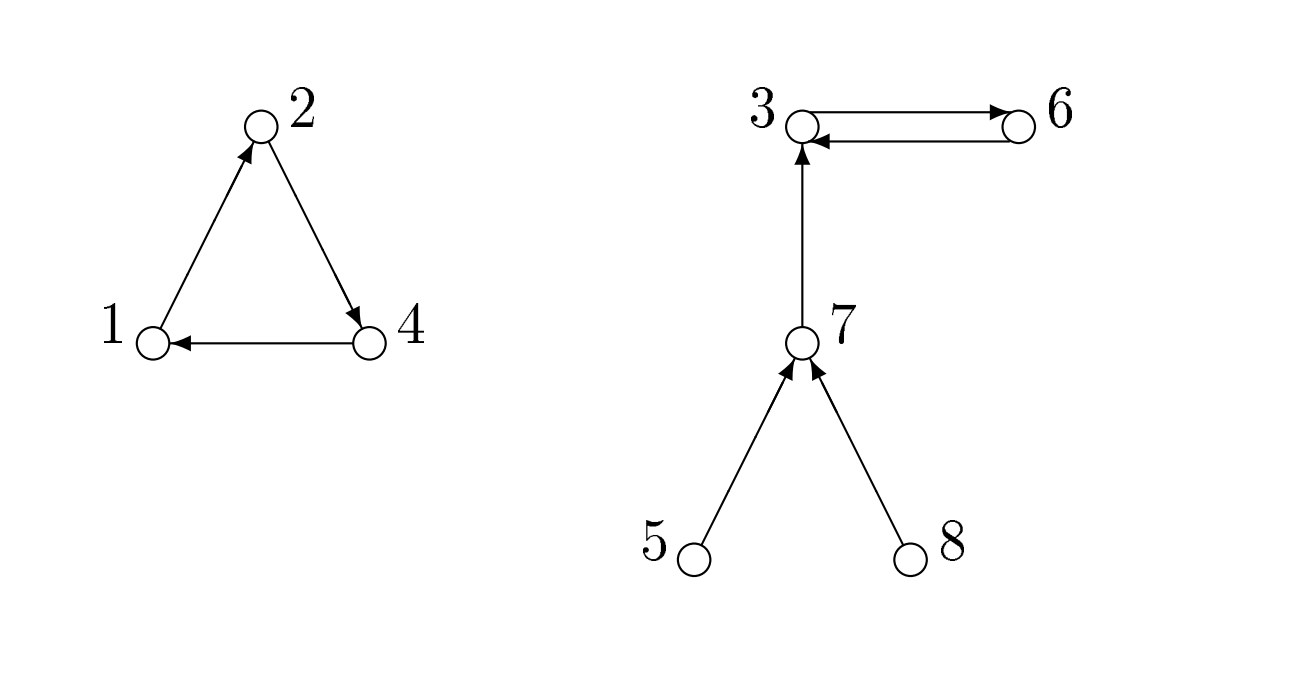
\includegraphics[width=0.65\textwidth]{IMAGES_FIGS/FIG_2_7.png}
  \caption{The graph $H(M)$}
  \label{FIG_3_3}
\end{figure}

The above proof gives a simple way to find a rotation exposed in $M$: starting from any man $m$, traverse the \textit{unique} path in $H(M)$ from $m$ until $m$ or some other node is visited twice. If $\rho$ is the rotation discovered by this traversal, we say that $m$ leads to rotation $\rho$; if $m$ leads to $\rho$ but is not in $\rho$, then the path in $H(M)$ from $m$ to the first man in $\rho$ is called a \textbf{tail} of $\rho$. Note that a rotation can have several tails. 

\begin{corollary}\label{cor_3_1}
If $m$ has different partners in $M$ and $M_z$, then $m$ leads to exactly one exposed rotation in $M$, so $m$ is either in exactly one rotation exposed in $M$ or is in exactly one tail.
\end{corollary}

The following lemma is an extension of Lemma \ref{lem_3_1} and is proved in essentially the same way.

\begin{lemma}\label{lem_3_4}
    If $\rho$ is exposed in $M$ and $m$ is a man on a tail of $\rho$ in $H(M)$, then $(m, w)$ cannot be a stable pair if $w$ is strictly between $p_M(m)$ and $s_M(m)$.
\end{lemma}



\section{Rotations and Minimal Differences}

In this section, we will exhibit a one-one correspondence between the rotations and the minimal differences of $\mathrm{P}(\mathcal{M})$. Then, given Lemma \ref{lem_3_2} and Lemma \ref{lem_3_3} above, and the fact that all the minimal differences are found along any maximal chain of $P(\mathcal{M})$, we will be able to identify all the minimal differences and all the rotations by successively finding and eliminating exposed rotations, myopicly following any maximal chain in $\mathcal{M}$ from $M_0$ to $M_z$. The following is a central technical lemma.

\begin{lemma}\label{lem_3_5}
If $M$ strictly dominates $M^{\prime}$, and $\rho$ is exposed in $M$, then either all the men in $\rho$ have the same partners in $M$ and in $M^{\prime}$, or none of them does. In the latter case, $M / \rho$ dominates $M^{\prime}$. Similarly, if a man $m$ is on a tail of $\rho$, and $m$ has different partners in the two matchings, then so does every man in $\rho$, and again $M / \rho$ dominates $M^{\prime}$.
\end{lemma}

\begin{proof}
By Lemma \ref{lem_3_1}, if $m_i \in \rho$ has a different partner $w$ in $M^{\prime}$ than in $M$, then $w$ must either be $s_M\left(m_i\right)$ or a woman below her in $m_i$ 's list. In either case, $s_M\left(m_i\right)$ must not be matched in $M^{\prime}$ to $m_{i+1}$, her partner in $M$, for if $s_M\left(m_i\right)$ and $m_{i+1}$ are partners in $M^{\prime}$, then either $s_M\left(m_i\right)$ has two partners in $M^{\prime}$, or the pair $\left(m_i,s_M\left(m_i\right)\right)$ blocks $M^{\prime}$. Hence $m_{i+1}$ must also have a different partner in $M^{\prime}$ than in $M$, and it follows that all men in $\rho$ have different partners in $M$ and $M^{\prime}$ if any one of them does. In the case that the men of $\rho$ have different partners in the two matchings, Lemma \ref{lem_3_1} implies that $M / \rho$ dominates (possibly equals) $M^{\prime}$, since the only men with different partners in $M$ and $M / \rho$ are the men in $\rho$. The case when $m$ is on a tail of $\rho$ is proved in essentially the same way, using Lemma \ref{lem_3_4} in place of Lemma \ref{lem_3_1}.
\end{proof}

\begin{exmp}\label{exmp_3_5}
In Figure \ref{FIG_2_2}, $M_1$ dominates both $M_4$ and $M_5$, among other matchings, and the rotation $(1,8),(2,3),(4,6)$, which we will call $\rho_1$, is exposed in $M_1$. In matching $M_5$, every man in $\rho_1$ has the same partner he has in $M_1$, while in $M_4$ every man in $\rho_1$ has a different partner. Further, $M_2=M_1 / \rho_1$ and $M_2$ dominates $M_4$, as required by the lemma.
\end{exmp}

\begin{theorem}\label{thm_3_1}
If $\rho$ is exposed in $M$, then $M$ is an immediate predecessor of $M / \rho$ in $\mathcal{M}$, and $P(M / \rho) \backslash P(M)$ is a minimal difference of $P(\mathcal{M})$.
\end{theorem}

\begin{proof}
    It is immediate from Lemma \ref{lem_3_5} that there is no stable matching $M^{\prime}$ such that $M$ dominates $M^{\prime}$, and $M^{\prime}$ dominates $M / \rho$, so $M$ immediately precedes $M / \rho$. Then by Lemma \ref{lem_2_11}, $P(M / \rho) \backslash P(M)$ is a minimal difference of $P(\mathcal{M})$.
\end{proof}

For rotation $\rho=\left(m_0, w_0\right),\left(m_1, w_1\right), \ldots,\left(m_{r-1}, w_{r-1}\right)$, we define $d(\rho)$ to be the set all pairs $\left(m_i, w\right)$, where $m_i \in \rho$ and $w$ is either $w_{i+1}$ or a woman strictly between $w_i$ and $w_{i+1}$ in $m_i$ 's list.

\begin{exmp}\label{exmp_3_6}
    When $\rho=(3,5),(6,1)$, which is a rotation in the example from Figure \ref{FIG_2_2}, then $m_0=3, m_1=6, w_0=5, w_1=1$, and so it can be seen from the preference lists of Figure \ref{FIG_2_1} that $d(\rho)=\{(3,1),(6,6),(6,7),(6,5)\}$
\end{exmp}

Notice that rotation $\rho$ is completely determined by the set of pairs $d(\rho)$ and the preference lists, and that $\rho$ can be constructed from $d(\rho)$ as follows: for each man $m$ in a pair $(m, w) \in d(\rho)$, let $w(m)$ be the woman $m$ most prefers among the women $w$ such that $(m, w)$ is in $d(\rho)$; let $\hat{w}(m)$ be the woman immediately before $w(m)$ in $m$ 's preference list. Then $\rho$ consists of all pairs $(m, \hat{w}(m))$, such that $m$ is in a pair $(m, w) \in d(\rho)$. The order of the pairs in $\rho$ is easily determined from these pairs and the preference lists.

\begin{lemma}\label{lem_3_6}
    If rotation $\rho$ is exposed in distinct matchings $M$ and $M^{\prime}$, then $P(M / \rho) \backslash P(M)=$ $P\left(M^{\prime} / \rho\right) \backslash P\left(M^{\prime}\right)=d(\rho)$.
\end{lemma}

\begin{proof}
    The difference $P(M / \rho) \backslash P(M)$ consists of all pairs $\left(m_i, w\right)$, where $w$ is either $w_{i+1}$ or a woman strictly between $w_i$ and $w_{i+1}$ in $m_i$ 's list. Clearly this set of pairs depends only on $\rho$ and the preference lists, and not on $M$. Hence, $P(M / \rho) \backslash P(M)=P\left(M^{\prime} / \rho\right) \backslash P\left(M^{\prime}\right)$, and they both are $d(\rho)$.
\end{proof}

Combining Lemma \ref{lem_3_6} and Theorem \ref{thm_3_1}, we have the following.

\begin{theorem}\label{thm_3_2}
    For any rotation $\rho$, the set of pairs $d(\rho)$ is a minimal difference of $P(\mathcal{M})$, and so each rotation $\rho$ maps to a unique minimal difference $d(\rho)$. Further, $d(\rho)$ can be constructed directly from $\rho$ and the preference lists.
\end{theorem}

%\begin{theo}
\begin{center}
\begin{minipage}{.8\linewidth}
\begin{algorithm}[H]
\caption{\textit{Minimal-differences}}
\begin{algorithmic}[1]
\State find the man and the woman-optimal matchings $M_0$, $M_z$;
\State $i:= 0$
\While {$M_i \neq M_z$}
\State Find an exposed rotation $\rho \in M_{i}$
\State $M_{i+1} := M_i/\rho_i$
\State $d(\rho_i) := P(M_{i+1}) \ P(M_i)$;
\EndWhile
\end{algorithmic}
\end{algorithm}
\end{minipage}

\begin{figure}[ht]
  \centering
  \caption{Algorithm to fnd all the minimal differences and rotations}
  \label{FIG_3_4}
\end{figure}
\end{center}
%\end{theo}

Our goal now is to show the converse of Theorem \ref{thm_3_2}, i.e., that every minimal difference of $P(\mathcal{M})$ is $d(\rho)$ for exactly one rotation $\rho$. We will do this through the use of Algorithm minimal differences, shown in Figure \ref{FIG_3_4}. This algorithm will find all the minimal differences of $P(\mathcal{M})$, and all the rotations of $\mathcal{M}$, using only the preference lists of the problem instance.

\begin{theorem}\label{thm_3_3}
    Every minimal difference of $P(\mathcal{M})$ is the set $d(\rho_i)$ for exactly one rotation $\rho_i$ generated by Algorithm minimal-differences and every rotation in $\mathcal{M}$ is generated exactly once by Algorithm minimal-differences.
    
\end{theorem}



\begin{proof}
    By Lemmas 2.5.2 and 2.5.3, each $M_i$ generated by the algorithm is a stable matching, and there is an exposed rotation in each matching until the woman optimal matching is reached. Further, by Theorem \ref{thm_3_1}, each $M_i$ is an immediate predecessor in $\mathcal{M}$ of $M_{i+1}$. Hence the sequence of st able matchings generated by the algorithm must be a maximal chain in $\mathcal{M}$ from the man optimal matching to the woman optimal matching. Now by Corollary \ref{cor_2_5}, every minimal difference of $\mathcal{M}$ appears exactly once as a consecutive difference of matchings along any maximal chain in $\mathcal{M}$; hence, every minimal difference of $\mathcal{M}$ is $d\left(\rho_i\right)$ for exactly one $\rho_i$ generated by the algorithm.
\end{proof}

For the second claim, let $\rho$ be any rotation, and let $M$ be any stable matching in which it is exposed. By Lemma \ref{lem_3_6} $d(\rho)=P(M / \rho) \backslash P(M)$, which is a minimal difference, by Theorem \ref{thm_3_1}. Hence $d(\rho)=d\left(\rho_i\right)$, for some $\rho_i$ found by the algorithm. But since $d(\rho)$ uniquely determines $\rho$, it follows that $\rho=\rho_i$.

Lets say that a rotation $\rho$ is on a chain in $\mathcal{M}$, and that the chain contains $\rho$, if the minimal difference $d(\rho)$ is on the corresponding chain in $P(\mathcal{M})$. Then, combining the results of this section with Theorem \ref{thm_2_1} we have the main result of this section.

\begin{theorem}\label{thm_3_4}
    There is a one-one correspondence $\rho \leftrightarrow d(\rho)$ between the rotations of $\mathcal{M}$ and the minimal differences of $P(\mathcal{M})$. Further, if $M$ dominates $M^{\prime}$, then every chain in $\mathcal{M}$ between $M$ and $M^{\prime}$ contains exactly the same set of rotations. Hence every rotation of $\mathcal{M}$ appears exactly once on every maximal chain of $\mathcal{M}$.
\end{theorem}
    
\begin{exmp}\label{exmp_3_7}
    Lets demonstrate Algorithm minimal-differences on the problem instance shown in Figure \ref{FIG_2_1}. In the example, we will use reduced preference lists. This will keep the lists smaller, and make it easier to recognize exposed rotations. Also, we will display only the reduced lists of the men, as all information can be extracted from their reduced lists. To verify that the reduced lists of the men are maintained correctly. To start, the $MGS$-lists for the man-optimal matching $M_0$ are shown in Figure \ref{FIG_3_5} 
\end{exmp}

\begin{center}
    $\begin{array}{llllllll}1: & 5 & 8 & 3 & & & & \\ 2: & 3 & 8 & 6 & & & & \\ 3: & 8 & 5 & 1 & 6 & 2 & & \\ 4: & 6 & 8 & 5 & & & & \\ 5: & 7 & 2 & 1 & 3 & 6 & 8 & 4 \\ 6: & 1 & 5 & 2 & 3 & & & \\ 7: & 2 & 5 & 7 & 8 & 1 & & \\ 8: & 4 & 5 & 2 & 6 & & & \end{array}$
    \begin{figure}[h]
  \centering
  \caption{ The $MGS$ lists}
  \label{FIG_3_5}
\end{figure}
\end{center}

\begin{exmp}\label{exmp_3_8}
    There is one exposed rotation $\rho_0=(1,5),(3,8)$ in $M_0$, and $M_0 / \rho_0=M_1$. The reduced lists for $M_1$ were used in an earlier example and appear in Figure \ref{FIG_3_2}. As noted before, there are two exposed rotations in $M_1$. Suppose the algorithm picks rotation $\rho_1=(1,8),(2,3),(4,6)$ at this point. Then $M_1 / \rho_1=M_2$; the reduced lists of the men for $M_2$ are shown in Figure \ref{FIG_3_6} .
\end{exmp}


\begin{exmp}\label{exmp_3_9}
    In $M_2$ there is one exposed rotation, $\rho_2=(3,5),(6,1)$, and $M_2 / \rho_2=M_4$ (note that we are using the name of the matching given in Figure \ref{FIG_2_2} rather than the name given by Algorithm minimal-differences). The reduced lists for $M_4$ are shown in Figure \ref{FIG_3_7}.
\end{exmp}

\begin{exmp}\label{exmp_3_10}
    The rotation $\rho_3=(7,2),(5,7)$ is exposed in $M_4$, and $M_4 / \rho_3=M_6$. The reduced lists are shown in Figure \ref{FIG_3_8}.
\end{exmp}

\begin{exmp}\label{exmp_3_11}
    Rotation $\rho_4=(3,1),(5,2)$ is exposed in $M_6$, and $M_6 / \rho_4=M_7$, the woman-optimal matching. The final reduced lists are shown in Figure \ref{FIG_3_9}.
\end{exmp}



\begin{center}
    $\begin{array}{llllll}1: & 3 & & & & \\ 2: & 6 & & & & \\ 3: & 5 & 1 & 2 & & \\ 4: & 8 & 5 & & & \\ 5: & 7 & 2 & 1 & & \\ 6: & 1 & 5 & 2 & & \\ 7: & 2 & 5 & 7 & 8 & 1 \\ 8: & 4 & 2 & & & \end{array}$
    \begin{figure}[ht]
  \centering
  \caption{The reduced lists of the men for stable matching $M_2$}
  \label{FIG_3_6}
\end{figure}
\end{center}


\begin{center}
    $\begin{array}{llll}1: & 3 & & \\ 2: & 6 & & \\ 3: & 1 & 2 & \\ 4: & 8 & & \\ 5: & 7 & 2 & 1 \\ 6: & 5 & 2 & \\ 7: & 2 & 7 & 8 \\ 8: & 4 & 2 & \end{array}$
    \begin{figure}[ht]
  \centering
  \caption{The reduced lists of the men for stable matching $M_4$}
  \label{FIG_3_7}
\end{figure}
\end{center}

\begin{center}
    $\begin{array}{lll}1: & 3 & \\ 2: & 6 & \\ 3: & 1 & 2 \\ 4: & 8 & \\ 5: & 2 & 1 \\ 6: & 5 & 2 \\ 7: & 7 & 8 \\ 8: & 4 & 2\end{array}$
    \begin{figure}[ht]
  \centering
  \caption{The reduced lists of the men for stable matching $M_6$}
  \label{FIG_3_8}
\end{figure}
\end{center}

\begin{center}
    $\begin{array}{lll}1: & 3 & \\ 2: & 6 & \\ 3: & 2 & \\ 4: & 8 & \\ 5: & 1 & \\ 6: & 5 & 2 \\ 7: & 7 & 8 \\ 8: & 4 & 2\end{array}$
    \begin{figure}[ht]
  \centering
  %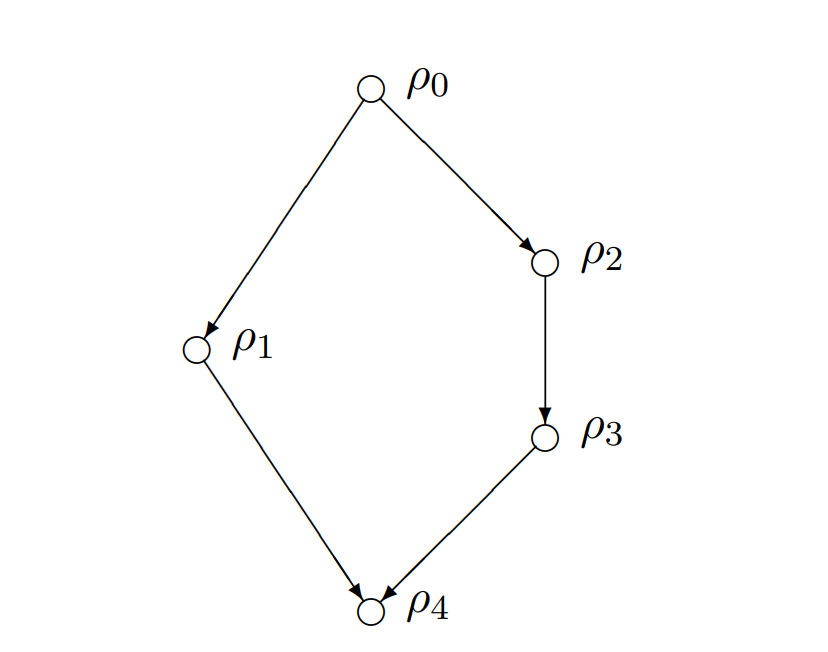
\includegraphics[width=0.5\textwidth]{IMAGES_FIGS/FIG_2_8.png}
  \caption{The reduced lists of the men for woman-optimal matching}
  \label{FIG_3_9}
\end{figure}
\end{center}



Even without additional implementation detail, it is easy to establish that Algorithm minimal differences needs no more than $O\left(n^3\right)$ time to find all the rotations. In the next chapter we will implement Algorithm minimal-differences to run in $O\left(n^2\right)$ time.

Any stable matching $M$ other than $M_z$ has an exposed rotation $\rho$ that defines a minimal difference $d(\rho)$, and both $\rho$ and $d(\rho)$ are easy to find from the reduced lists for $M$. Hence rotations allow one to focus on a single stable matching $M$, knowing that $d(\rho)$ is a minimal difference of $\mathcal{M}$, whereas the definition of a minimal difference involves a very particular stable matching, an irreducible one, or involves two stable matchings. The existence of rotations is the special, algorithmically valuable feature of $P(\mathcal{M})$ that does not exist in a general ring of sets.



\section{The Rotations Generate All Stable Matchings}
We know that the minimal differences of $P(\mathcal{M})$ can be used to generate all the stable matchings, and that the rotations can be used to generate the minimal differences. Hence, the rotations can surely be used to generate all the stable matchings. In this section we will establish a more direct approach to thinking about and using rotations for this purpose.

\begin{lemma}\label{lem_3_7}
    Let $M$ be an immediate predecessor of $M^{\prime}$ in $\mathcal{M}$, and let $\rho$ be the rotation such that $d(\rho)=P\left(M^{\prime}\right) \backslash P(M)$. Then $\rho$ is exposed in $M$, and $M / \rho=M^{\prime}$.
\end{lemma}

\begin{proof}
    It is immediate from the definition of $d(\rho)$, and the way that $\rho$ is uniquely determined from $d(\rho)$, that if $\rho$ is exposed in $M$, then $M^{\prime}=M / \rho$. Every man $m^{\prime} \in \rho$ has different partners in $M$ and $M_z$, so by Corollary 2.5.1, $m^{\prime}$ leads to some rotation $\rho^{\prime}$ exposed in $M$. Now since $m^{\prime}$ has a different partner in $M$ than in $M^{\prime}$, Lemma \ref{lem_3_5} implies that each man $m \in \rho^{\prime}$ must also have different partners in $M^{\prime}$ and $M$. Let $w$ be $m$ 's partner in $M$, and let $w^{\prime}$ be the woman just following $w$ in $m$ 's list. Then $\left(m, w^{\prime}\right)$ must be in the minimal difference $P\left(M^{\prime}\right) \backslash P(M)=d(\rho)$. But $\left(m, w^{\prime}\right)$ must also be in $d\left(\rho^{\prime}\right)$, so it must be that $d(\rho)=d\left(\rho^{\prime}\right)$ which can only happen when $\rho^{\prime}=\rho$, hence $\rho$ is exposed in $M$.
\end{proof}

\begin{corollary}\label{cor_3_2}
    For any stable matchings $M$ and $M^{\prime}$, where $M$ dominates $M^{\prime}$, let $C$ be a chain between $M$ and $M^{\prime}$ in $\mathcal{M}$. Then $M^{\prime}$ can be generated from $M$ by successively exposing and eliminating the rotations on $C$, in their order on $C$. Further, every sequence of rotation eliminations transforming $M$ to $M^{\prime}$ contains exactly the same set of rotations, although in a different order.
\end{corollary}

\begin{proof}
    The first statement follows inductively from Lemma \ref{lem_3_7}. The second statement follows from the fact that any sequence of rotation eliminations follows a chain in $\mathcal{M}$, and Theorem \ref{thm_2_1}.
\end{proof}

Specializing Corollary \ref{cor_3_2} to the case when $M=M_0$ gives the next theorem.

\begin{theorem}\label{thm_3_5}
    Every stable matching $M^{\prime}$ can be generated by a sequence of rotation eliminations, starting from $M_0$, and every such sequence contains exactly the same rotations.
\end{theorem}

That is, chains in $\mathcal{M}$ not only indicate how to transform one matching to another by unioning the minimal differences along the corresponding chain in $P(\mathcal{M})$, but they also indicate how to transform matchings by successive rotation eliminations.

\begin{exmp}\label{exmp_3_12}
    Every edge in Figure \ref{FIG_2_2} is labeled with the name of one of the rotations obtained by Algorithm minimal-differences. If $M$ is an immediate predecessor of $M^{\prime}$, then the edge $\left(M, M^{\prime}\right)$ is labeled with the rotation $\rho$ such that $d(\rho)=P\left(M^{\prime}\right) \backslash P(M)$. Corollary \ref{cor_3_2} is very clearly illustrated in that figure.
\end{exmp}

\subsection{Characterizing stable pairs}

At this point, we have the tools to characterize the stable pairs of any problem instance.

\begin{theorem}\label{thm_3_6}
    \begin{itemize}
        \item A pair $(m, w)$ is a stable pair if and olly if it is a pair in $M_z$ or it is a pair in some rotation. Equivalently, $(m, w)$ is stable if and only if it is a pair in $M_0$, or for some rotation $\left(m_0, w_0\right),\left(m_1, w_1\right), \ldots,\left(m_{r-1}, w_{r-1}\right)$ and some $i, m=m_i$ and $w=w_{i+1}$.
        \item  A pair is a fixed pair if and only if it is in both $M_0$ and $M_z$, or equivalently, it is in $M_0$ but not in any rotation.
    \end{itemize}
\end{theorem}

\begin{proof}
    \begin{itemize}
        \item The "if" part is by definition. For the "only if" part, let $(m, w)$ be a stable pair in a stable matching $M \neq M_z$. Then by Corollary \ref{cor_3_2} , there is a chain $C$ in $\mathcal{M}$ from $M$ to $M_z$, and $M_z$ can be obtained by eliminating the rotations on this chain in order. Since $p_{M_z}(m) \neq w$, there must be some rotation $\rho$ on $C$ whose elimination changes $m$ 's partner from $w$ to some other woman. But then, $(m, w)$ must be in $\rho$.
        \item The proof of is immediate.
    \end{itemize}
\end{proof}

By Theorem \ref{thm_3_4}, every rotation is contained on every maximal chain in $\mathcal{M}$, so combined with Theorem \ref{thm_3_6} we have the following observation.

\begin{corollary}\label{cor_3_3}
The stable matchings on any maximal chain in $\mathcal{M}$ contain all the stable pairs of $\mathcal{M}$
\end{corollary}


\section{The Rotation Poset} 

Given the one-one correspondence between the minimal differences of $P(\mathcal{M})$ and the rotations of $\mathcal{M}$, we can finally define the long awaited representation $\Pi(\mathcal{M})$ of $\mathcal{M}$ based on rotations.

\begin{figure}[ht]
  \centering
  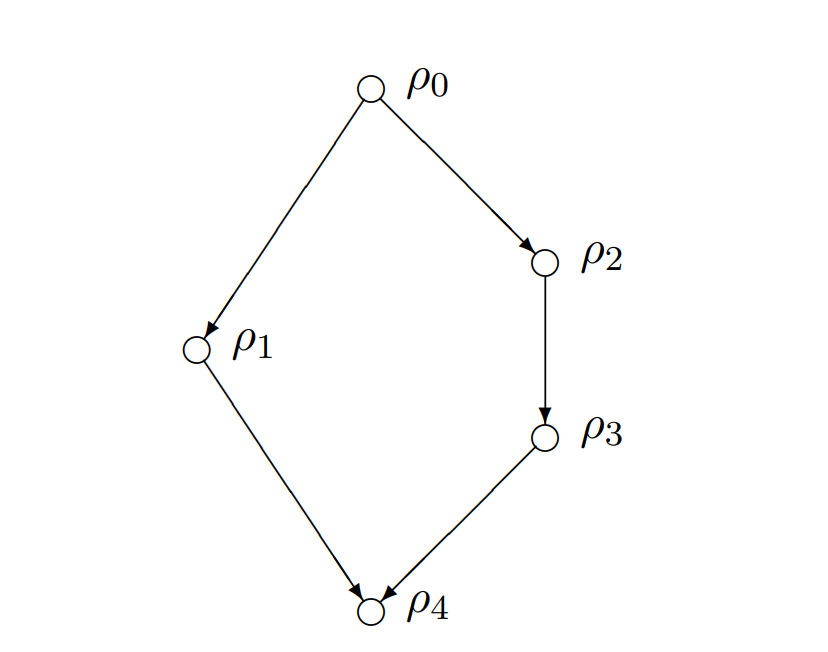
\includegraphics[width=0.4\textwidth]{IMAGES_FIGS/FIG_2_8.png}
  \caption{The rotation poset for $\mathcal{M}$}
  \label{FIG_3_10}
\end{figure}

The rotation poset of $\mathcal{M}$, denoted $\Pi(\mathcal{M})$, is the partial or der on the rotations of $\mathcal{M}$ defined by replacing each minimal difference $d(\rho)$ in the partial order $D(\mathcal{M})$ by the rotation $\rho$. The precedence relation on $\Pi(\mathcal{M})$ corresponds exactly to that on $D(\mathcal{M}): \rho^{\prime}$ precedes $\rho$ in $\Pi(\mathcal{M})$ if and only if $d\left(\rho^{\prime}\right)$ precedes $d(\rho)$ in $D(\mathcal{M})$. Note that $\Pi(\mathcal{M})$ is isomorphic to the partial order $I(\mathcal{M})$ after the removal of $M_0$ from $I(\mathcal{M})$.

\begin{theo}
    \begin{itemize}
        \item There is a one-one correspondence between the closed subsets of $\Pi(\mathcal{M})$ and the stable matchings of $\mathcal{M}$.
        \item $S$ is the closed set of rotations of $\Pi(\mathcal{M})$ corresponding to a stable matching $M$ if and only if $S$ is the (unique) set of rotations on every $M_0$-chain in $\mathcal{M}$ ending at $M$. Further, $M$ can be generated from $M_0$ by eliminating the rotations in their order along any of these paths, and these are the only ways to generate $M$ by rotation eliminations starting from $M_0$.
        \item If $S$ and $S^{\prime}$ are the unique sets of rotations corresponding to distinct stable matchings $M$ and $M^{\prime}$, then $M$ dominates $M^{\prime}$ if and only if $S \subset S^{\prime}$.
    \end{itemize}
\end{theo} 


\bibliographystyle{unsrt}
\bibliography{bib.bib}
\end{document}
